%<<echo=FALSE>>=
%OLD <- options(width=90)
%@
%<<echo=FALSE>>=
%options(OLD) 
%@

\documentclass{beamer}\usepackage[]{graphicx}\usepackage[]{color}
%% maxwidth is the original width if it is less than linewidth
%% otherwise use linewidth (to make sure the graphics do not exceed the margin)
\makeatletter
\def\maxwidth{ %
  \ifdim\Gin@nat@width>\linewidth
    \linewidth
  \else
    \Gin@nat@width
  \fi
}
\makeatother

\definecolor{fgcolor}{rgb}{0.102, 0.102, 0.102}
\newcommand{\hlnum}[1]{\textcolor[rgb]{0.2,0.2,0.2}{#1}}%
\newcommand{\hlstr}[1]{\textcolor[rgb]{0.2,0.2,0.2}{#1}}%
\newcommand{\hlcom}[1]{\textcolor[rgb]{0.302,0.302,0.302}{\textit{#1}}}%
\newcommand{\hlopt}[1]{\textcolor[rgb]{0.102,0.102,0.102}{#1}}%
\newcommand{\hlstd}[1]{\textcolor[rgb]{0.102,0.102,0.102}{#1}}%
\newcommand{\hlkwa}[1]{\textcolor[rgb]{0.102,0.102,0.102}{#1}}%
\newcommand{\hlkwb}[1]{\textcolor[rgb]{0.102,0.102,0.102}{#1}}%
\newcommand{\hlkwc}[1]{\textcolor[rgb]{0.2,0.2,0.2}{#1}}%
\newcommand{\hlkwd}[1]{\textcolor[rgb]{0.102,0.102,0.102}{\textbf{#1}}}%

\usepackage{framed}
\makeatletter
\newenvironment{kframe}{%
 \def\at@end@of@kframe{}%
 \ifinner\ifhmode%
  \def\at@end@of@kframe{\end{minipage}}%
  \begin{minipage}{\columnwidth}%
 \fi\fi%
 \def\FrameCommand##1{\hskip\@totalleftmargin \hskip-\fboxsep
 \colorbox{shadecolor}{##1}\hskip-\fboxsep
     % There is no \\@totalrightmargin, so:
     \hskip-\linewidth \hskip-\@totalleftmargin \hskip\columnwidth}%
 \MakeFramed {\advance\hsize-\width
   \@totalleftmargin\z@ \linewidth\hsize
   \@setminipage}}%
 {\par\unskip\endMakeFramed%
 \at@end@of@kframe}
\makeatother

\definecolor{shadecolor}{rgb}{.97, .97, .97}
\definecolor{messagecolor}{rgb}{0, 0, 0}
\definecolor{warningcolor}{rgb}{1, 0, 1}
\definecolor{errorcolor}{rgb}{1, 0, 0}
\newenvironment{knitrout}{}{} % an empty environment to be redefined in TeX

\usepackage{alltt}% regular slides (with pauses)
%\documentclass[handout]{beamer}% handout (no pauses)

%%%%%%%%%%%%%%%%%%%%%%%%%%%%%%%%%%%%%%%%%%%%%%%%%%%%%%%%%%%%%%%%%%%%%%%%%
%%%%%%% Change the lecture information here %%%%%%%%%%%%%%%%
\def\chapnum{Week \#1}
\title{STAT234: Lecture 4 - Continuing with Probability !!}
\author{Kushal K. Dey}
\date{}
%%%%%%%%%%%%%%%%%%%%%%%%%%%%%%%%%%%%%%%%%%%%%%%%%%%%%%%%%%%%%%%%%%%%%%%%%

%%%%%% Start of suggested definitions and packages %%%%%%%%%%%%
%%%%%% Do not change unless you really know what you are doing %%%%%%%%%%
%%%%%%%%%%%%%%%%%%%%%%%%%%%%%%%%%%%%%%%%%%%%%%%%%%%%%%%%%%%%%%%%%%%%%%%%%

\usepackage{enumerate}
\usepackage{amsmath, bbm}
\usepackage[misc]{ifsym} % for the dice symbol \Cube{}
\usepackage[latin1]{inputenc}
\usepackage{hyperref}

%\usepackage{comment}
%\usepackage{pstricks}
%\usepackage{graphicx}
%\usepackage{booktabs}
%\usepackage{pgfpages}
%\pgfpagesuselayout{2 on 1}[a4paper,border shrink=3mm]
%\pgfpagesuselayout{4 on 1}[a4paper,landscape,border shrink=3mm

\usepackage{setspace}
\ifdefined\knitrout
  \renewenvironment{knitrout}{\begin{spacing}{0.75}\begin{tiny}}{\end{tiny}\end{spacing}}
\else
\fi

%%%%%%%%%%%%%%% Defined Shortcuts (macros) %%%%%%%%%%%%%
% parameters and statistics
\newcommand{\xbar}{\overline{x}}
\newcommand{\Xbar}{\overline{X}}
\newcommand{\ybar}{\overline{y}}
\newcommand{\Ybar}{\overline{Y}}
\newcommand{\dbar}{\overline{d}}
\newcommand{\Dbar}{\overline{D}}
\newcommand{\zbar}{\overline{z}}
\newcommand{\Zbar}{\overline{Z}}
\newcommand{\ehat}{\widehat{\epsilon}}
\newcommand{\yhat}{\widehat{y}}
\newcommand{\Yhat}{\widehat{Y}}
\newcommand{\betaa}{{\beta_0}}
\newcommand{\betab}{{\beta_1}}
\newcommand{\betac}{{\beta_2}}
\newcommand{\betad}{{\beta_3}}
\newcommand{\BETA}{{\boldsymbol\beta}}
\newcommand{\betahata}{\widehat{\beta_0}}
\newcommand{\betahatb}{\widehat{\beta_1}}
\newcommand{\betahatc}{\widehat{\beta_2}}
\newcommand{\betahatd}{\widehat{\beta_3}}
\newcommand{\bhat}{\widehat{b}}
\newcommand{\btilde}{\widetilde{b}}
\newcommand{\ahat}{\widehat{a}}
\newcommand{\atilde}{\widetilde{a}}
\newcommand{\rss}{\mathit{SSE}}
\newcommand{\sigmahat}{\widehat{\sigma}}
\newcommand{\betahat}{\widehat{\beta}}
\newcommand{\thetahat}{\widehat{\theta}}
\newcommand{\phat}{\widehat{p}}
\newcommand{\pihat}{\widehat{\pi}}
\newcommand{\muhat}{\widehat{\mu}}
% real numbers and integers
\newcommand{\reals}{\mathbbm{R}}
\newcommand{\integers}{\mathbbm{N}}
%distributions
\newcommand{\normal}{\textsf{Norm}}
\newcommand{\Bin}{\textsf{Binom}}
\newcommand{\Uni}{\textsf{Unif}}
\newcommand{\Poisson}{\textsf{Pois}}
\newcommand{\Exp}{\textsf{Exp}}
\newcommand{\Beta}{\textsf{Beta}}
\newcommand{\iid}{\stackrel{\mathrm{iid}}{\sim}}
% probability and expected value
\newcommand{\rv}{r.v.\ }
\newcommand{\prob}{{\rm P}}
\newcommand{\mean}{\mathrm{E}}
\newcommand{\var}{\mathrm{Var}}
\newcommand{\Var}{\mathrm{Var}}
\newcommand{\cov}{\mathrm{Cov}}
\newcommand{\corr}{\mathop{\mathrm{Corr}}}
% measures of spread
\newcommand{\IQR}{\textit{IQR}}
\newcommand{\SAD}{\textit{SAD}}
\newcommand{\MAD}{\textit{MAD}}
\newcommand{\SSD}{\textit{SSD}}
\newcommand{\MSD}{\textit{MSD}}
\newcommand{\RMSD}{\textit{RMSD}}
\newcommand{\MSE}{\textit{MSE}}
\newcommand{\MSR}{\textit{MSR}}
% formatting code and such
\providecommand{\variable}[1]{}
\renewcommand{\variable}[1]{{\color{green!50!black}\texttt{#1}}}
\providecommand{\function}[1]{}
\renewcommand{\function}[1]{{\color{purple!75!blue}\texttt{\StrSubstitute{#1}{()}{}()}}}
\providecommand{\option}[1]{}
\renewcommand{\option}[1]{{\color{brown!80!black}\texttt{#1}}}
\providecommand{\pkg}[1]{}
\renewcommand{\pkg}[1]{{\color{red!80!black}\texttt{#1}}}
\providecommand{\code}[1]{}
\renewcommand{\code}[1]{{\color{blue!80!black}\texttt{#1}}}

%%%%%%%%%
% Changed by Kushal K Dey, University of Chicago
%\providecommand{\file}[1]{}
%\renewcommand{\file}[1]{{\tt #1}}
\providecommand{\file}[1]{}
\renewcommand{\file}[1]{{\color{orange!80!black}\texttt{#1}}}
%\providecommand{\dataframe}[1]{}
%\renewcommand{\dataframe}[1]{{\color{blue!80!black}\texttt{#1}}}
\providecommand{\dataframe}[1]{}
\renewcommand{\dataframe}[1]{{\color{cyan!80!black}\texttt{#1}}}
%%%%%%%%%

% other
\def\Sum{\sum\nolimits}
\def\b#1{\fboxsep=0pt\colorbox{black}{\color{white}\Cube{#1}}}
\def\w#1{\Cube{#1}}
%%%%%%%%%%%% End of shortcuts (macros) ##############

%%%%%%%%% One way to hide answers until you want to show them %%%%%%%%%
\def\Hide#1#2{\ul{~~~\onslide<#1>{\alert{#2}}~~~}}
\def\hide#1#2{\ul{~~\onslide<#1>{\alert{#2}}~~}}
\def\hid#1#2{\onslide<#1>{\alert{#2}}}
% Choose the color of answers here too
\setbeamercolor{alerted text}{fg=darkgray} 
%\setbeamercolor{alerted text}{fg=black} 

%------Centered Page Number Setup ------
\defbeamertemplate{footline}{centered page number}
{%
  \hspace*{\fill}%
  %\usebeamercolor[fg]{page number in head/foot}%
  %\usebeamerfont{page number in head/foot}%
  \tiny \chapnum: Page \insertframenumber\, of \inserttotalframenumber%
  \hspace*{\fill}\vskip2pt%
}
%\setbeamertemplate{footline}{\hfill\insertframenumber/\inserttotalframenumber}
\setbeamertemplate{footline}[centered page number]
%--------------------------------

%\usetheme{Copenhagen}
\setbeamertemplate{navigation symbols}{}
\usepackage[english]{babel}
\def\ul{\underline}
\linespread{1.1}
% or whatever



%\parskip=0pt
\IfFileExists{upquote.sty}{\usepackage{upquote}}{}
\begin{document}%large

%<<setup, include=FALSE, cache=FALSE>>=
%options(replace.assign=TRUE,width=90, digits=4)
%opts_chunk$set(fig.path='figure/graphics-', cache.path='cache/graphics-', fig.align='center', fig.width=8, fig.height=4.5, fig.show='as.is', out.width='0.9\\linewidth', cache=FALSE, par=TRUE, size = 'tiny', tidy=TRUE, cache.extra=rand_seed)
%knit_hooks$set(par=function(before, options, envir){
%if (before && options$fig.show!='none') par(mar=c(4,4,.1,.1),cex.lab=.95,cex.axis=.9,mgp=c(2,.7,0),tcl=-.3)
%}, document = function(x) {
%  gsub('\\\\(begin|end)\\{kframe\\}', '', x)
%}, crop=hook_pdfcrop)
%@
%<<setup2, include=FALSE, cache=FALSE>>=
%knit_theme$set("print")
%@


%%%%%%%%%%%%%%%%%%%%%%%%%%%%%%%%%%%%%%%%%%%%%%%%%%%%%%%%%%%%%%%%%%%%%%%%%
%%%%%%%%%%%%%%%%%%%%%%%%%%%%%%%%%%%%%%%%%%%%%%%%%%%%%%%%%%%%%%%%%%%%%%%%%
%%%%%% End of suggested definitions and packages %%%%%%%%%%%%

%------------------------------------------------------------------
%------------------------------------------------------------------

%%%%%%%%%% Title frame (optional) %%%%%%%%%%%%%
\begin{frame}{}
\maketitle
\end{frame}
%%%%%%%%%%%%%%%%%%%%%%%%%%%%%%%%%%%%%%%%%%%%%%%

%%%%%%%%%%%%%% Begin slides here %%%%%%%%%%%%%%

%%%%%%%%%%%%%%%%%%%%%%%%%%%%%%%%%%%%%%%%%%%%%%%%%%%%%%%%%%%%
\begin{frame}[fragile]{Notion of independence \;\;}
%%%%%%%%%%%%%%%%%%%%%%%%%%%%%%%%%%%%%%%%%%%%%%%%%%%%%%%%%%%%

Consider two tosses of a fair coin. \pause \newline

Tosses are independent (as per textbook definition). \pause \newline

Is that consistent with mathematical definition of independence?

Define $X1$ to be $1$ if first toss gives H, $0$ otherwise.

Define $X2$ to be $1$ if second toss gives H, $0$ otherwise.

\end{frame}
%%%%%%%%%%%%%%%%%%%%%%%%%%%%%%%%%%%%%%%%%%%%%%%%%%%%%%%%%%%%


%%%%%%%%%%%%%%%%%%%%%%%%%%%%%%%%%%%%%%%%%%%%%%%%%%%%%%%%%%%%
\begin{frame}[fragile]{Independent variables \;\;}
%%%%%%%%%%%%%%%%%%%%%%%%%%%%%%%%%%%%%%%%%%%%%%%%%%%%%%%%%%%%


\begin{tabular}{|c|c|c|c|}
\hline
state & $X_1$ & $X_2$ & Prob\\ \hline
HH & 1 & 1 & 0.25\\ \hline
HT & 1 & 0 & 0.25\\ \hline
TH & 0 & 1 & 0.25\\ \hline
TT & 0 & 0 & 0.25\\ \hline
\end{tabular} \pause \newline \newline

\begin{tabular}{|c|c|c|}
\hline
$X1|X2$ & 0 & 1 \\ \hline 
0 &  0.25 &  0.25 \\ \hline
1 &  0.25 &  0.25 \\ \hline
\end{tabular} \pause \newline \newline


$$ Pr[X_1=0, X_2=0] = 0.25 $$
\end{frame}
%%%%%%%%%%%%%%%%%%%%%%%%%%%%%%%%%%%%%%%%%%%%%%%%%%%%%%%%%%%%



%%%%%%%%%%%%%%%%%%%%%%%%%%%%%%%%%%%%%%%%%%%%%%%%%%%%%%%%%%%%
\begin{frame}[fragile]{Independent variables \;\;}
%%%%%%%%%%%%%%%%%%%%%%%%%%%%%%%%%%%%%%%%%%%%%%%%%%%%%%%%%%%%

Row marginal distribution (distribution of X1)

\begin{tabular}{|c|c|c|c|}
\hline
$X1|X2$ & 0 & 1  & \textcolor{red}{Total}\\ \hline 
0 &  0.25 &  0.25  & \textcolor{red}{0.50}\\ \hline
1 &  0.25 &  0.25  & \textcolor{red}{0.50}\\ \hline
 & & & \textcolor{red}{1} \\ \hline
\end{tabular} \pause \newline

$$ Pr[X_1=0] = Pr[X_1 = 1] =0.5 $$

Column marginal distribution (distribution of X2) \pause \newline

\begin{tabular}{|c|c|c|c|}
\hline
$X1|X2$ & 0 & 1  & \\ \hline 
0 &  0.25 &  0.25  & \\ \hline
1 &  0.25 &  0.25  & \\ \hline
\textcolor{red}{Total} & \textcolor{red}{0.50} & \textcolor{red}{0.50} &  \textcolor{red}{1} \\ \hline
\end{tabular} \pause \newline 

$$ Pr[X_2=0] = Pr[X_2 = 1] =0.5 $$
\end{frame}
%%%%%%%%%%%%%%%%%%%%%%%%%%%%%%%%%%%%%%%%%%%%%%%%%%%%%%%%%%%%


%%%%%%%%%%%%%%%%%%%%%%%%%%%%%%%%%%%%%%%%%%%%%%%%%%%%%%%%%%%%
\begin{frame}[fragile]{Independent variables \;\;}
%%%%%%%%%%%%%%%%%%%%%%%%%%%%%%%%%%%%%%%%%%%%%%%%%%%%%%%%%%%%

Check that 

$$ Pr[ X_1=0, X_2 =0 ] =0.25 = 0.5 \times 0.5 = Pr [X_1 = 0] \times Pr [X_2 =0] $$ \newline
$$ Pr[ X_1=1, X_2 =0 ] =0.25 = 0.5 \times 0.5 = Pr [X_1 = 1] \times Pr [X_2 =0] $$ \newline
$$ Pr[ X_1=0, X_2 =1 ] =0.25 = 0.5 \times 0.5 = Pr [X_1 = 0] \times Pr [X_2 =1] $$ \newline
$$ Pr[ X_1=1, X_2 =1 ] =0.25 = 0.5 \times 0.5 = Pr [X_1 = 1] \times Pr [X_2 =1] $$ \newline

This shows independence because for all realizations $x$ of $X_1$ (namely 0 and 1) and 
all realizations $y$ of $X_2$ (namely 0 and 1)

$$ Pr [X_1 =x, X_2 = y] = Pr [X_1 =x ] \times Pr [X_2=y] $$
\end{frame}
%%%%%%%%%%%%%%%%%%%%%%%%%%%%%%%%%%%%%%%%%%%%%%%%%%%%%%%%%%%%

%%%%%%%%%%%%%%%%%%%%%%%%%%%%%%%%%%%%%%%%%%%%%%%%%%%%%%%%%%%%
\begin{frame}[fragile]{Conditionality \;\;}
%%%%%%%%%%%%%%%%%%%%%%%%%%%%%%%%%%%%%%%%%%%%%%%%%%%%%%%%%%%%

Define conditional probability as 

$$ Pr[X_2 = y | X_1 = x] : =  \frac{Pr [X_1 = x, X_2 = y]} {Pr [X_1 =x]} $$

Then I get 

$$ Pr [ X_1 = x, X_2 = y] = Pr [X_1 = x] \times Pr[X_2 = y | X_1 = x] $$

unless $ Pr [X_1 =x] = 0$.

We abbreviate this as 

$$ p_{XY}(x,y) = p_{Y|X}(y|x) p_{X}(x) $$

\end{frame}
%%%%%%%%%%%%%%%%%%%%%%%%%%%%%%%%%%%%%%%%%%%%%%%%%%%%%%%%%%%%

%%%%%%%%%%%%%%%%%%%%%%%%%%%%%%%%%%%%%%%%%%%%%%%%%%%%%%%%%%%%
\begin{frame}[fragile]{Conditionality \;\;}
%%%%%%%%%%%%%%%%%%%%%%%%%%%%%%%%%%%%%%%%%%%%%%%%%%%%%%%%%%%%

What happens to conditionality under independence 

\begin{align}
Pr [X_2 = y | X_1 =x ] & = \frac{Pr [X_1 = x, X_2 = y]} {Pr [X_1 =x]} \\
& = \frac{Pr [X_1 = x] \times Pr [X_2 =y]}{ Pr [X_1 = x]} \\
& = Pr[ X_2 = y] \\
\end{align}

So under independence, for any realization $x$ and $y$

$$ Pr [X_2 = y | X_1 =x ] = Pr[X_2 = y] $$

\end{frame}
%%%%%%%%%%%%%%%%%%%%%%%%%%%%%%%%%%%%%%%%%%%%%%%%%%%%%%%%%%%%

%%%%%%%%%%%%%%%%%%%%%%%%%%%%%%%%%%%%%%%%%%%%%%%%%%%%%%%%%%%%
\begin{frame}[fragile]{Conditionality \;\;}
%%%%%%%%%%%%%%%%%%%%%%%%%%%%%%%%%%%%%%%%%%%%%%%%%%%%%%%%%%%%

\begin{tabular}{|c|c|c|c|}
\hline
$X1|X2$ & 0 & 1  & \textcolor{red}{Total}\\ \hline 
0 &  0.25 &  0.25  & \textcolor{red}{0.50}\\ \hline
1 &  0.25 &  0.25  & \textcolor{red}{0.50}\\ \hline
 & & & \textcolor{red}{1} \\ \hline
\end{tabular} \pause \newline


Conditional distribution of $X1$
\begin{tabular}{|c|c|c|c|}
\hline
$X1|X2$ & 0 & 1  & \\ \hline 
0 &  0.25/0.50 = 0.5 &  0.25/0.50 = 0.5 & 1\\ \hline
1 &  0.25/0.50 = 0.5 &  0.25/0.50 = 0.5  & 1\\ \hline
\end{tabular} \pause \newline 

$$ Pr[X_2 = 0 | X_1 = 0] = 0.5 = Pr [X_2 = 0] $$

\end{frame}
%%%%%%%%%%%%%%%%%%%%%%%%%%%%%%%%%%%%%%%%%%%%%%%%%%%%%%%%%%%%

%%%%%%%%%%%%%%%%%%%%%%%%%%%%%%%%%%%%%%%%%%%%%%%%%%%%%%%%%%%%
\begin{frame}[fragile]{Independence implies? \;\;}
%%%%%%%%%%%%%%%%%%%%%%%%%%%%%%%%%%%%%%%%%%%%%%%%%%%%%%%%%%%%

Independence of two random variables $X$ and $Y$ implies the following

\begin{itemize}
\item $p_{XY}(x,y) = Pr [ X=x, Y=y] = Pr [X=x] \times Pr [Y=y] = p_{X}(x) p_{Y}(y) \forall x, y $ \pause \newline
\item $p_{Y|X}(y|x) = Pr [ Y=y | X=x ] = Pr [Y=y] = p_{Y}(y)  \forall x, y $ \pause  \newline
\item $ E(XY) = E(X)E(Y) $  \pause \newline
\item $ cov(X,Y) = E(XY) - E(X)E(Y) = 0 $  \pause \newline
\item $ var (X + Y) = var(X) + var(Y) $  \pause \newline
\item $ var (X - Y) = var(X) + var(Y) $ \pause \newline
\end{itemize}

\end{frame}
%%%%%%%%%%%%%%%%%%%%%%%%%%%%%%%%%%%%%%%%%%%%%%%%%%%%%%%%%%%%


%%%%%%%%%%%%%%%%%%%%%%%%%%%%%%%%%%%%%%%%%%%%%%%%%%%%%%%%%%%%
\begin{frame}[fragile]{Example of Non-independence  \;\;}
%%%%%%%%%%%%%%%%%%%%%%%%%%%%%%%%%%%%%%%%%%%%%%%%%%%%%%%%%%%%

\begin{center}
\begin{tabular}{l|c||c|c|c||c|}
\multicolumn{5}{c}{$X$}\\
\cline{2-6}
&&0&1&2&$p(y)$\\
\cline{2-6}
$Y$&0&2/6& 1/6&0&3/6\\
\cline{2-6}
   &1&0&1/6&2/6&3/6\\
\cline{2-6}
   &$p(x)$ &2/6&2/6&2/6&\\
\cline{2-6}
\end{tabular}
\end{center}

Consider the pair $(x,y,) = (0,0).$
$$p(0,0) = 2/6 \ne p_X(0)p_Y(0) = (1/3)(1/2) = 1/6.$$

$X$ and $Y$ are not independent.

\end{frame}
%%%%%%%%%%%%%%%%%%%%%%%%%%%%%%%%%%%%%%%%%%%%%%%%%%%%%%%%%%%%


%%%%%%%%%%%%%%%%%%%%%%%%%%%%%%%%%%%%%%%%%%%%%%%%%%%%%%%%%%%%
\begin{frame}{Sums of Random Variables}
%%%%%%%%%%%%%%%%%%%%%%%%%%%%%%%%%%%%%%%%%%%%%%%%%%%%%%%%%%%%

Suppose we consider 3 independent tosses of a coin 

\begin{tabular}{|c|c|c|c|c|c|}
\hline
state & $X_1$ & $X_2$ & $X_3$ & $Y=X_1 + X_2 + X_3$ & Prob\\ \hline
HHH & 1 & 1 & 1 & 3 & $p^3$ \\ \hline
HHT & 1 & 1 & 0 & 2 & $p^2 (1-p) $ \\ \hline
HTH & 1 & 0 & 1 & 2 & $p^2 (1-p) $ \\ \hline
HTT & 1 & 0 & 0 & 1 & $p (1-p)^2 $ \\ \hline
THH & 0 & 1 & 1 & 2 & $p^2 (1-p) $\\ \hline
THT & 0 & 1 & 0 & 1 & $ p (1-p)^2 $ \\ \hline
TTH & 0 & 0 & 1 & 1 & $ p (1-p)^2 $ \\ \hline
TTT & 0 & 0 & 0 & 0 & $ (1-p)^3 $ \\ \hline
\end{tabular} \pause \newline \newline
 \end{frame}
%%%%%%%%%%%%%%%%%%%%%%%%%%%%%%%%%%%%%%%%%%%%%%%%%%%%%%%%%%%%

%%%%%%%%%%%%%%%%%%%%%%%%%%%%%%%%%%%%%%%%%%%%%%%%%%%%%%%%%%%%
\begin{frame}{Distribution of Y}
%%%%%%%%%%%%%%%%%%%%%%%%%%%%%%%%%%%%%%%%%%%%%%%%%%%%%%%%%%%%

\begin{tabular}{|c|c|}
\hline
Y & Prob  \\ \hline
3 & $p^3$ \\ \hline
2 & $3 p^2 (1-p) $ \\ \hline
1 & $3 p (1-p)^2 $\\ \hline
0 & $ (1-p)^3 $\\ \hline
\end{tabular} \pause \newline

Have we seen these probabilities before? \pause \newline

What about $ Bin(3, p) $. \pause \newline

That means $ Y \sim Bin(3, p) $.  \pause \newline

Can we make this more general?

 \end{frame}
%%%%%%%%%%%%%%%%%%%%%%%%%%%%%%%%%%%%%%%%%%%%%%%%%%%%%%%%%%%%

%%%%%%%%%%%%%%%%%%%%%%%%%%%%%%%%%%%%%%%%%%%%%%%%%%%%%%%%%%%%
\begin{frame}{Bernoulli and Binomial connection}
%%%%%%%%%%%%%%%%%%%%%%%%%%%%%%%%%%%%%%%%%%%%%%%%%%%%%%%%%%%%

If $X_1, X_2, \cdots, X_n$ be $n$ independently generated random variables such that 

$$ X_{i} \sim Ber(p) \;\; \forall i $$

There is another notation for this 

$$ X_{i} \stackrel{iid}{\sim} Ber(p) $$

then we define 

$$ Y = X_1 + X_2 + \cdots + X_n $$

then we have 

$$ Y \sim Bin(n,p)  $$

 \end{frame}
%%%%%%%%%%%%%%%%%%%%%%%%%%%%%%%%%%%%%%%%%%%%%%%%%%%%%%%%%%%%

%%%%%%%%%%%%%%%%%%%%%%%%%%%%%%%%%%%%%%%%%%%%%%%%%%%%%%%%%%%%
\begin{frame}[fragile]{Moment generating function \;\;}
%%%%%%%%%%%%%%%%%%%%%%%%%%%%%%%%%%%%%%%%%%%%%%%%%%%%%%%%%%%%

The moment generating function (Mgf) is given by

\begin{align}
Mgf(t) & : = E(e^{tX}) \\
& = E \left ( \left \{ \sum_{k=1}^{\infty} \frac{(tX)^{k}}{k!} \right \} Pr(X=k) \right) \\
& = \sum_{k=1}^{K} \frac{t^{k}}{k!} E \left ( X^{k} \right) \\
& = \sum_{k=1}^{K} \frac{t^{k}}{k!} \mu_{k}
\end{align}

$\mu_{k}$ is called the $k$th moment of the distribution of $X$. 

\end{frame}
%%%%%%%%%%%%%%%%%%%%%%%%%%%%%%%%%%%%%%%%%%%%%%%%%%%%%%%%%%%%


%%%%%%%%%%%%%%%%%%%%%%%%%%%%%%%%%%%%%%%%%%%%%%%%%%%%%%%%%%%%
\begin{frame}{Moment generating function}
%%%%%%%%%%%%%%%%%%%%%%%%%%%%%%%%%%%%%%%%%%%%%%%%%%%%%%%%%%%%

The moment generating function of a random variable $X$ evaluated at $t$

$$ Mgf (t) = E \left ( e^{tX} \right) $$

Suppose we want to calculate the moment generating function for sums of random variables that are independent ($Z=X+Y$ where $X,Y$ independent).

\begin{align}
Mgf_{X+Y}(t) & = E \left ( e^{t(X+Y)} \right ) \\
       & = E \left ( e^{tX}e^{tY} \right)  \\
       & = E \left ( e^{tX} \right) E \left ( e^{tY} \right) \\
       & = Mgf_X(t) Mgf_Y(t) \\
\end{align}

 \end{frame}
%%%%%%%%%%%%%%%%%%%%%%%%%%%%%%%%%%%%%%%%%%%%%%%%%%%%%%%%%%%%

%%%%%%%%%%%%%%%%%%%%%%%%%%%%%%%%%%%%%%%%%%%%%%%%%%%%%%%%%%%%
\begin{frame}{Moment generating function}
%%%%%%%%%%%%%%%%%%%%%%%%%%%%%%%%%%%%%%%%%%%%%%%%%%%%%%%%%%%%

If $X$ and $Y$ have the same distribution, say $Ber(p)$,

$$ Mgf_{X}(t) = Mgf_{Y}(t) = Mgf(t)  $$ \pause \newline

Now assume there are $n$ independent random variables with same distribution instead of two. \pause

$$ Mgf_{X_1 + X_2 + \cdots X_{n}}(t) = \left [ Mgf(t) \right]^{n} $$ \pause

We can use this relationship to get the Mgf of the Binomial distribution from the Mgf of the Bernoulli distribution. \pause \newline 

What are the Mgf, mean and variance of Binomial distribution?

 \end{frame}
%%%%%%%%%%%%%%%%%%%%%%%%%%%%%%%%%%%%%%%%%%%%%%%%%%%%%%%%%%%%

%%%%%%%%%%%%%%%%%%%%%%%%%%%%%%%%%%%%%%%%%%%%%%%%%%%%%%%%%%%%
\begin{frame}{Variance of sum}
%%%%%%%%%%%%%%%%%%%%%%%%%%%%%%%%%%%%%%%%%%%%%%%%%%%%%%%%%%%%

Note from the Bernoulli and Binomial connection that $ Y \sim Bin(n,p)$ can be writen as 

$$ Y = X_1 + X_2 + \cdots + X_{n} $$

where $X_i$ is $Ber(p)$ and all the $X_i$ are independent 

We showed that 

$$ var(Y) = np (1-p) $$

and 

$$ var(X_i) = p(1-p) $$

This validates 

$$ var(Y) = var(X_1) + var(X_2) + \cdots + var(X_n) $$

where all $X_i$ are independent.

\end{frame}
%%%%%%%%%%%%%%%%%%%%%%%%%%%%%%%%%%%%%%%%%%%%%%%%%%%%%%%%%%%%

%%%%%%%%%%%%%%%%%%%%%%%%%%%%%%%%%%%%%%%%%%%%%%%%%%%%%%%%%%%%
\begin{frame}{Relations of Variance and Expectation}
%%%%%%%%%%%%%%%%%%%%%%%%%%%%%%%%%%%%%%%%%%%%%%%%%%%%%%%%%%%%

From the definition you can show

\begin{itemize}
\item $E(c)=c$ and $var(c)=0$ \pause \newline
\item $E(X+Y)= E(X) + E(Y) $ and $ var(X+Y) = var(X) + var(Y) + 2cov(X,Y)$. The result 
$ var(X+Y) = var(X) + var(Y) $ holds under independence of $X$ and $Y$. Converse not true.
\pause \newline
\item $ E(aX) = a E(X)$ and $ var(aX) = a^2 var(X) $ \pause \newline
\item $ E(aX+ bY) = aE(X) + bE(Y)$ and $ var(aX+bY) = a^2 var(X) + b^2 var(Y) + 2ab cov(X,Y)$ and under independence $ var(aX + bY) = a^2 var(X) + b^2 var(Y) $ \pause \newline
\end{itemize}
\end{frame}
%%%%%%%%%%%%%%%%%%%%%%%%%%%%%%%%%%%%%%%%%%%%%%%%%%%%%%%%%%%%

%%%%%%%%%%%%%%%%%%%%%%%%%%%%%%%%%%%%%%%%%%%%%%%%%%%%%%%%%%%%
\begin{frame}{Last relation: Expectation}
%%%%%%%%%%%%%%%%%%%%%%%%%%%%%%%%%%%%%%%%%%%%%%%%%%%%%%%%%%%%

\begin{align*}
&E(aX+bY) = \sum_x \sum_y
               (ax+by) p(x,y)\\
&\hid{2-}{=  \sum_x \sum_y ax p(x,y) + \sum_x \sum_y by p(x,y)}\\
&\hid{2-}{=  \sum_x \sum_y ax p(x,y) + \sum_y \sum_x by p(x,y)}\\
&\hid{3-}{= \sum_x ax
\underbrace{\left[\sum_y p(x,y)\right]}_{\hid{4-}{=p_X(x)}} + \sum_y by
\underbrace{\left[\sum_x p(x,y)\right]}_{\hid{5-}{=p_Y(y)}}\;\;*}\\
&\hid{6-}{= a \sum_x x p_X(x) + b \sum_y y  p_Y(y)}
\hskip2.5cm \hid{7-}{= aE(X) + bE(Y)}
\end{align*}
\hid{3-}{{\small{*\; See HW0 for more details about the ``double sum."}}}

\end{frame}
%%%%%%%%%%%%%%%%%%%%%%%%%%%%%%%%%%%%%%%%%%%%%%%%%%%%%%%%%%%%

%%%%%%%%%%%%%%%%%%%%%%%%%%%%%%%%%%%%%%%%%%%%%%%%%%%%%%%%%%%%
\begin{frame}{Sums of Random Variables}
%%%%%%%%%%%%%%%%%%%%%%%%%%%%%%%%%%%%%%%%%%%%%%%%%%%%%%%%%%%%

$$ E(X+Y) =  E(X) + E(Y) $$

$$ E(X + Y + Z) = E(X+Y) + E(Z) = E(X) + E(Y) + E(Z) $$

$$ E( X_1 + X_2 + \cdots + X_n ) = E(X_1) + E(X_2) + \cdots + E(X_n) $$

$$ E( a_1X_1 + a_2X_2 + \cdots + a_nX_n ) = a_1E(X_1) + a_2E(X_2) + \cdots + a_nE(X_n) $$

$$ E \left ( \sum_{i=1}^{n} a_iX_i \right ) = \sum_{i=1}^{n} a_i E(X_{i}) $$

 \end{frame}
%%%%%%%%%%%%%%%%%%%%%%%%%%%%%%%%%%%%%%%%%%%%%%%%%%%%%%%%%%%%

%%%%%%%%%%%%%%%%%%%%%%%%%%%%%%%%%%%%%%%%%%%%%%%%%%%%%%%%%%%%
\begin{frame}{Means of Random Variables}
%%%%%%%%%%%%%%%%%%%%%%%%%%%%%%%%%%%%%%%%%%%%%%%%%%%%%%%%%%%%

$$ E \left ( \sum_{i=1}^{n} a_iX_i \right ) = \sum_{i=1}^{n} a_i E(X_{i}) $$

Assume $a_i = \frac{1}{n}$ for all $i$,

$$ E \left ( \frac{1}{n} \sum_{i=1}^{n} X_i \right ) = \sum_{i=1}^{n} \frac{1}{n} E(X_{i}) $$

Suppose all $X_i$ are from same distribution, then 

$$ E(X_1) = E(X_2) = \cdots = E(X_n) = E(X)= \mu$$

 \end{frame}
%%%%%%%%%%%%%%%%%%%%%%%%%%%%%%%%%%%%%%%%%%%%%%%%%%%%%%%%%%%%

%%%%%%%%%%%%%%%%%%%%%%%%%%%%%%%%%%%%%%%%%%%%%%%%%%%%%%%%%%%%
\begin{frame}{Means of Random Variables}
%%%%%%%%%%%%%%%%%%%%%%%%%%%%%%%%%%%%%%%%%%%%%%%%%%%%%%%%%%%%

$$ E \left ( \frac{1}{n} \sum_{i=1}^{n} X_i \right ) = \sum_{i=1}^{n} \frac{1}{n} E(X_{i}) $$

$$ E(X_1) = E(X_2) = \cdots = E(X_n) = E(X)= \mu$$

$$ E \left ( \frac{1}{n} \sum_{i=1}^{n} X_i \right ) = \sum_{i=1}^{n} \frac{1}{n} \mu $$

$$ E \left ( \frac{1}{n} \sum_{i=1}^{n} X_i \right ) = \mu $$

What does this mean? 

If I repeat the experiment of drawing n samples man computing the $\bar{X}_{n}$ many many times, then on an average these $\bar{X}_{n}$ will lie around the model/population mean $\mu$.

 \end{frame}
%%%%%%%%%%%%%%%%%%%%%%%%%%%%%%%%%%%%%%%%%%%%%%%%%%%%%%%%%%%%

%%%%%%%%%%%%%%%%%%%%%%%%%%%%%%%%%%%%%%%%%%%%%%%%%%%%%%%%%%%%
\begin{frame}{Unbiasedness}
%%%%%%%%%%%%%%%%%%%%%%%%%%%%%%%%%%%%%%%%%%%%%%%%%%%%%%%%%%%%

For random variables $X_1, X_2, \cdots, X_n$, all of which are coming from same distribution with mean $E(X_i)=\mu$ for all $i$,  we say a function $f(X_1, X_2, \cdots, X_n)$
is unbiased for $\mu$ if 

$$ E \left [f(X_1, X_2, \cdots, X_n) \right ] =  \mu$$

In the previous case, 

$$ f(X_1, X_2, \cdots, X_n) = \frac{1}{n} \sum_{i=1}^{n} X_{i}  $$

But the mean of the random varables may not be the only function that is unbiased for 
$\mu$. 

\end{frame}
%%%%%%%%%%%%%%%%%%%%%%%%%%%%%%%%%%%%%%%%%%%%%%%%%%%%%%%%%%%%


%%%%%%%%%%%%%%%%%%%%%%%%%%%%%%%%%%%%%%%%%%%%%%%%%%%%%%%%%%%%
\begin{frame}{Last relation: Variance}
%%%%%%%%%%%%%%%%%%%%%%%%%%%%%%%%%%%%%%%%%%%%%%%%%%%%%%%%%%%%

$$ var(a_1X_1+ a_2 X_2 + \cdots + a_nX_n) = \sum_{i=1}^{n} a^2_{i} var (X_{i}) $$ \pause

This implies 

$$ var \left (\frac{X_1 + X_2 + \cdots + X_{n}}{n} \right ) = \frac{1}{n^2} \left (var(X_1 + var(X_2) + \cdots + var(X_n)) \right ) $$ \pause

When all $X_i$ come from same distribution

$$ var(X_1) = var(X_2) = \cdots = var(X_n) = \sigma^2 $$ \pause 

$$ var \left (\frac{X_1 + X_2 + \cdots + X_{n}}{n} \right ) = \frac{1}{n^2} \left (\sigma^2 + \sigma^2 + \cdots + \sigma^2 \right) $$

\end{frame}
%%%%%%%%%%%%%%%%%%%%%%%%%%%%%%%%%%%%%%%%%%%%%%%%%%%%%%%%%%%%

%%%%%%%%%%%%%%%%%%%%%%%%%%%%%%%%%%%%%%%%%%%%%%%%%%%%%%%%%%%%
\begin{frame}{Last relation: Variance}
%%%%%%%%%%%%%%%%%%%%%%%%%%%%%%%%%%%%%%%%%%%%%%%%%%%%%%%%%%%%

$$ var(a_1X_1+ a_2 X_2 + \cdots + a_nX_n) = \sum_{i=1}^{n} a^2_{i} var (X_{i}) $$

This implies 

$$ var \left (\frac{X_1 + X_2 + \cdots + X_{n}}{n} \right ) = \frac{1}{n^2} \left (var(X_1 + var(X_2) + \cdots + var(X_n)) \right ) $$

When all $X_i$ come from same distribution

$$ var(X_1) = var(X_2) = \cdots = var(X_n) = \sigma^2 $$

$$ var \left (\frac{X_1 + X_2 + \cdots + X_{n}}{n} \right ) = \frac{1}{n^2}(n \sigma^2) $$

\end{frame}
%%%%%%%%%%%%%%%%%%%%%%%%%%%%%%%%%%%%%%%%%%%%%%%%%%%%%%%%%%%%

%%%%%%%%%%%%%%%%%%%%%%%%%%%%%%%%%%%%%%%%%%%%%%%%%%%%%%%%%%%%
\begin{frame}{Last relation: Variance}
%%%%%%%%%%%%%%%%%%%%%%%%%%%%%%%%%%%%%%%%%%%%%%%%%%%%%%%%%%%%

$$ var(a_1X_1+ a_2 X_2 + \cdots + a_nX_n) = \sum_{i=1}^{n} a^2_{i} var (X_{i}) $$ 

This implies 

$$ var \left (\frac{X_1 + X_2 + \cdots + X_{n}}{n} \right ) = \frac{1}{n^2} \left (var(X_1 + var(X_2) + \cdots + var(X_n)) \right ) $$ 

When all $X_i$ come from same distribution

$$ var(X_1) = var(X_2) = \cdots = var(X_n) = \sigma^2 $$

$$ var \left (\bar{X}_{n} \right ) = \frac{\sigma^2}{n} $$

\end{frame}
%%%%%%%%%%%%%%%%%%%%%%%%%%%%%%%%%%%%%%%%%%%%%%%%%%%%%%%%%%%%

%%%%%%%%%%%%%%%%%%%%%%%%%%%%%%%%%%%%%%%%%%%%%%%%%%%%%%%%%%%%
\begin{frame}{Expectation of $\bar{X}$ for Bernoulli}
%%%%%%%%%%%%%%%%%%%%%%%%%%%%%%%%%%%%%%%%%%%%%%%%%%%%%%%%%%%%

If all $X_{i}$ are independent $Ber(p)$ distribution (each $X_i$ is 1/0 with prob p or (1-p)), then 

$$ E(X_1) = E(X_2) = \cdots = E(X_n) = p $$

$p$ is the population mean of $Ber(p)$, then as per previous discussion,

$$ E(\frac{1}{n} \sum_{i=1}^{n} X_i) = p $$

Now here there is another way of viewing the mean of the $X_i$, it is the proportion of heads you get in $n$ trials, so we call it \textit{sampling proportion} 

$$ \hat{p} = \frac{1}{n} \sum_{i=1}^{n} X_i $$

\end{frame}
%%%%%%%%%%%%%%%%%%%%%%%%%%%%%%%%%%%%%%%%%%%%%%%%%%%%%%%%%%%%


%%%%%%%%%%%%%%%%%%%%%%%%%%%%%%%%%%%%%%%%%%%%%%%%%%%%%%%%%%%%
\begin{frame}{Variance of $\bar{X}$ for Bernoulli}
%%%%%%%%%%%%%%%%%%%%%%%%%%%%%%%%%%%%%%%%%%%%%%%%%%%%%%%%%%%%

If all $X_{i}$ are independent $Ber(p)$ distribution, then 

$$ var(X_1) = var(X_2) = \cdots = var(X_n) = p(1-p) $$ \pause \newline

Define 

$$ Y = X_1 + X_2 + \cdots + X_n$$, \pause

we can write

$$ var(\hat{p}) = var (\bar{X}_{n}) = var \left (\frac{1}{n} \sum_{i=1}^{n} X_{i} \right) = \frac{p(1-p)}{n} $$

\end{frame}
%%%%%%%%%%%%%%%%%%%%%%%%%%%%%%%%%%%%%%%%%%%%%%%%%%%%%%%%%%%%

%%%%%%%%%%%%%%%%%%%%%%%%%%%%%%%%%%%%%%%%%%%%%%%%%%%%%%%%%%%%
\begin{frame}{Summary of  $\bar{X}$ }
%%%%%%%%%%%%%%%%%%%%%%%%%%%%%%%%%%%%%%%%%%%%%%%%%%%%%%%%%%%%

For random variables $X_1, X_2, \cdots, X_n$, independently generated and coming from same distribution with mean and variance of the population given by 

$$ E(X_i) = \mu \hspace{1 cm} var(X_i) = \sigma^2  $$

Then if we compute $ \bar{X}_{n} = \frac{1}{n} \sum_{i=1}^{n} X_i$,

$$ E(\bar{X}_{n}) = \mu  \hspace{1 cm} var(\bar{X}_{n}) = \frac{\sigma^2}{n}  $$

For Bernoulli distribution,

$$ E(\bar{X}_{n}) = p  \hspace{1 cm} var(\bar{X}_{n}) = \frac{p(1-p)}{n}  $$

\end{frame}
%%%%%%%%%%%%%%%%%%%%%%%%%%%%%%%%%%%%%%%%%%%%%%%%%%%%%%%%%%%%



% %%%%%%%%%%%%%%%%%%%%%%%%%%%%%%%%%%%%%%%%%%%%%%%%%%%%%%%%%%%%
% \begin{frame}{Covariance between Random Variables}
% %%%%%%%%%%%%%%%%%%%%%%%%%%%%%%%%%%%%%%%%%%%%%%%%%%%%%%%%%%%%
% 
% The covariance between random variables $X$ and $Y$ is defined as
% 
% \begin{align}
% cov(X,Y)  & = E(X- E(X)(Y-E(Y)))  \\
%           &  = E(XY - E(X)Y - XE(Y) + E(X)E(Y)) \\
%           &  = E(XY) - E(E(X)Y) - E(XE(Y)) + E(E(X)E(Y)) \\
%           &  = E(XY) - E(X)E(Y) - E(X)E(Y) + E(X)E(Y) \\
%           &  = E(XY) - E(X)E(Y) \\
%           &  = \sum_{x,y} xy Pr(X=x, Y=y) - E(X)E(Y) \\
% \end{align} \pause
% 
% When $X$ and $Y$ are independent, we also have $cov(X,Y)=0$ \pause \newline
% 
% The converse is not true!!
% \end{frame}
% %%%%%%%%%%%%%%%%%%%%%%%%%%%%%%%%%%%%%%%%%%%%%%%%%%%%%%%%%%%%
% 
% %%%%%%%%%%%%%%%%%%%%%%%%%%%%%%%%%%%%%%%%%%%%%%%%%%%%%%%%%%%%
% \begin{frame}{Example to disprove the converse}
% %%%%%%%%%%%%%%%%%%%%%%%%%%%%%%%%%%%%%%%%%%%%%%%%%%%%%%%%%%%%
% 
% Let $X$ be a random variable
% 
% \begin{align}
% X & = 1 \;\; prob \;\; 0.5
%   & = -1 \;\; prob \;\; 0.5
% \end{align}
% 
% Let $Y$ be another random variable
% \begin{align}
% Y & = 0 \;\; if \; X=1 \\
%   & = +1 \;\; if \; X=-1 \; prob \; 0.5 \\
%   & = -1 \;\; if \; X=-1 \; prob \; 0.5 \\
%  \end{align}
% 
%  Then check that $E(XY)=E(X)=E(Y)=0$ and so $cov(X,Y)=0$
% 
%  Show $X$ and $Y$ are not independent
% 
%  \end{frame}
% %%%%%%%%%%%%%%%%%%%%%%%%%%%%%%%%%%%%%%%%%%%%%%%%%%%%%%%%%%%%
% 
% %%%%%%%%%%%%%%%%%%%%%%%%%%%%%%%%%%%%%%%%%%%%%%%%%%%%%%%%%%%%
% \begin{frame}{Properties of covariance}
% %%%%%%%%%%%%%%%%%%%%%%%%%%%%%%%%%%%%%%%%%%%%%%%%%%%%%%%%%%%%
% 
% \begin{itemize}
% \item $cov(X,X)= var(X)$ \pause \newline
% \item $cov(c, X)=0$ where $c$ is a constant variable, $X$ any other r.v.  \pause \newline
% \item $cov(aX, Y) = a \times cov(X,Y)$ where $a$ is a constant. \pause \newline
% \item $cov(aX, bY)= ab \times cov(X,Y)$ where $a,b$ are constants. \pause \newline
% \item $cov(aX + cZ, bY) = ab \times cov(X,Y) + bc \times cov(Z,Y)$ 
% \end{itemize}
% 
% \end{frame}
% %%%%%%%%%%%%%%%%%%%%%%%%%%%%%%%%%%%%%%%%%%%%%%%%%%%%%%%%%%%%

%%%%%%%%%%%%%%%%%%%%%%%%%%%%%%%%%%%%%%%%%%%%%%%%%%%%%%%%%%%%
\begin{frame}{Lets go back to Bernoulli}
%%%%%%%%%%%%%%%%%%%%%%%%%%%%%%%%%%%%%%%%%%%%%%%%%%%%%%%%%%%%

Suppose $X_1, X_2, \cdots, X_n$ are independent random variables coming from $Ber(p)$ distribution. \pause \newline

What do we know about it? \pause \newline

\begin{itemize}
\item $Y = \sum_{i=1}^{n} X_{i}$ follows $Bin(n,p)$ distribution. \pause
\item $E \left (\frac{1}{n} \sum_{i=1}^{n} X_{i} \right ) = p $ \pause
\item $ var \left (\frac{1}{n} \sum_{i=1}^{n} X_{i} \right ) = \frac{p(1-p)}{n} $ \pause
\item $ E(Y) = np$ and $var(Y) = np(1-p)$ (both from mgf and variance rule of sum of random variables) \pause
\end{itemize}

Lets repeat the experiment of generating $n$ samples many many times.

\end{frame}
%%%%%%%%%%%%%%%%%%%%%%%%%%%%%%%%%%%%%%%%%%%%%%%%%%%%%%%%%%%%

%%%%%%%%%%%%%%%%%%%%%%%%%%%%%%%%%%%%%%%%%%%%%%%%%%%%%%%%%%%%
\begin{frame}[fragile]
%%%%%%%%%%%%%%%%%%%%%%%%%%%%%%%%%%%%%%%%%%%%%%%%%%%%%%%%%%%%
\frametitle{Repeat of experiments}

Let us start with a simple example where we repeat the experiment of tossing
$100$ fair coins and recording the number of heads $10$ times.

\begin{knitrout}\small
\definecolor{shadecolor}{rgb}{1, 1, 1}\color{fgcolor}\begin{kframe}
\begin{alltt}
\hlstd{Y} \hlkwb{<-} \hlkwd{rbinom}\hlstd{(}\hlnum{10}\hlstd{,} \hlnum{100}\hlstd{,} \hlkwc{p}\hlstd{=}\hlnum{0.5}\hlstd{)}
\hlstd{Y}
\end{alltt}
\begin{verbatim}
 [1] 47 49 55 48 55 58 47 46 48 55
\end{verbatim}
\end{kframe}
\end{knitrout}

\end{frame}
%%%%%%%%%%%%%%%%%%%%%%%%%%%%%%%%%%%%%%%%%%%%%%%%%%%%%%%%%%%%

%%%%%%%%%%%%%%%%%%%%%%%%%%%%%%%%%%%%%%%%%%%%%%%%%%%%%%%%%%%%
\begin{frame}[fragile]
%%%%%%%%%%%%%%%%%%%%%%%%%%%%%%%%%%%%%%%%%%%%%%%%%%%%%%%%%%%%

\begin{knitrout}\small
\definecolor{shadecolor}{rgb}{1, 1, 1}\color{fgcolor}

{\centering 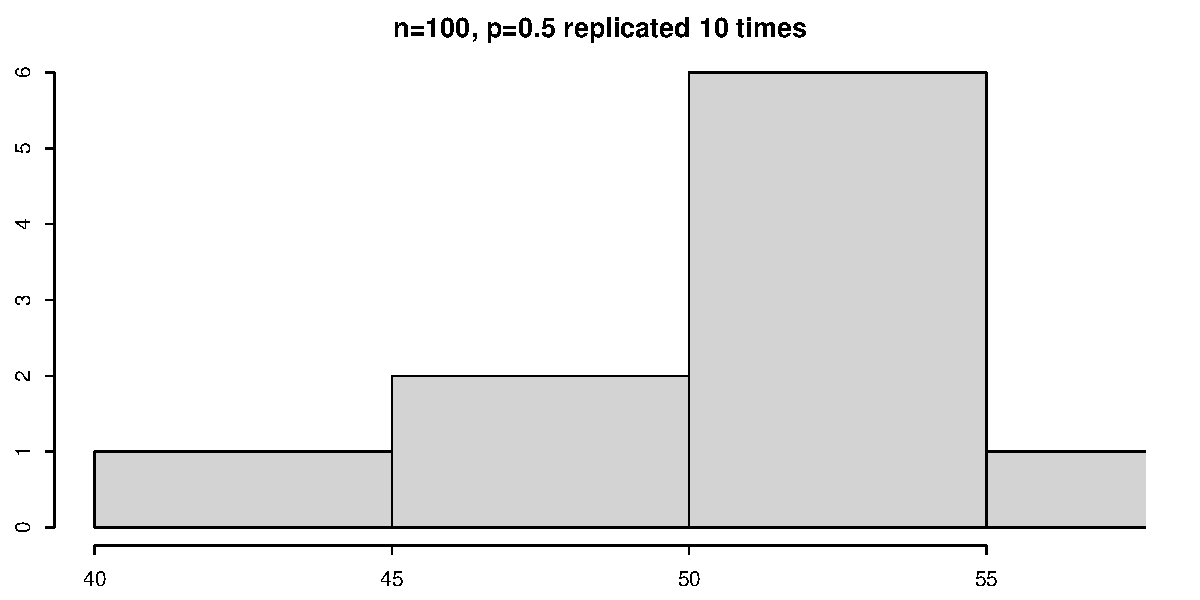
\includegraphics[width=0.89\linewidth]{figure/graphics-unnamed-chunk-2-1} 

}



\end{knitrout}

\end{frame}
%%%%%%%%%%%%%%%%%%%%%%%%%%%%%%%%%%%%%%%%%%%%%%%%%%%%%%%%%%%%

%%%%%%%%%%%%%%%%%%%%%%%%%%%%%%%%%%%%%%%%%%%%%%%%%%%%%%%%%%%%
\begin{frame}[fragile]
%%%%%%%%%%%%%%%%%%%%%%%%%%%%%%%%%%%%%%%%%%%%%%%%%%%%%%%%%%%%

\begin{knitrout}\small
\definecolor{shadecolor}{rgb}{1, 1, 1}\color{fgcolor}

{\centering 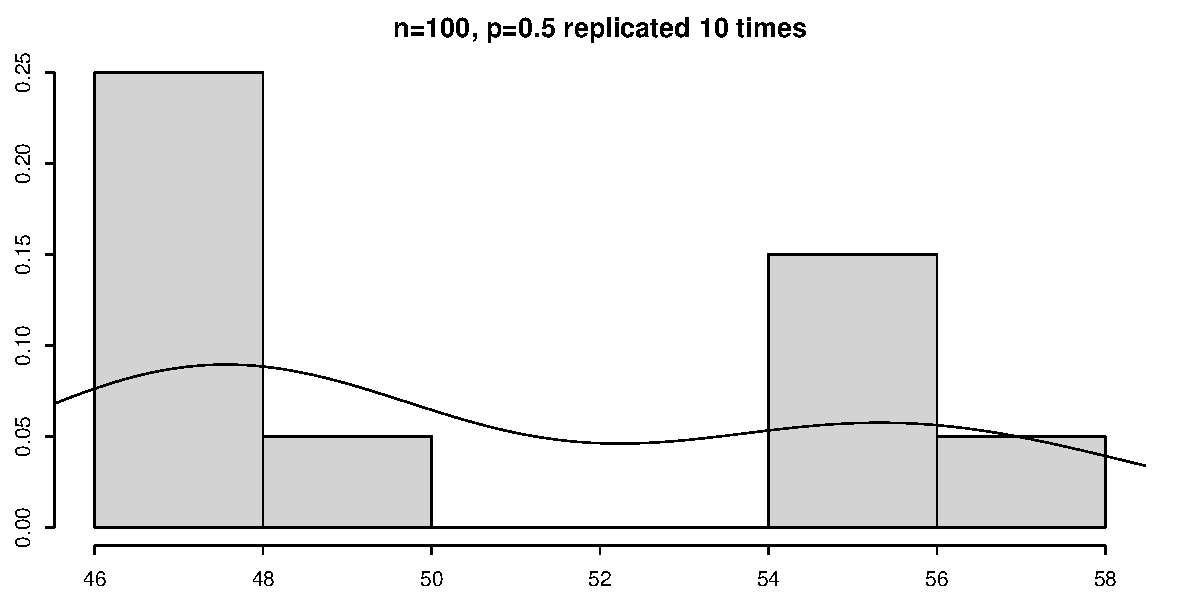
\includegraphics[width=0.89\linewidth]{figure/graphics-unnamed-chunk-3-1} 

}



\end{knitrout}

\end{frame}
%%%%%%%%%%%%%%%%%%%%%%%%%%%%%%%%%%%%%%%%%%%%%%%%%%%%%%%%%%%%

%%%%%%%%%%%%%%%%%%%%%%%%%%%%%%%%%%%%%%%%%%%%%%%%%%%%%%%%%%%%
\begin{frame}[fragile]
%%%%%%%%%%%%%%%%%%%%%%%%%%%%%%%%%%%%%%%%%%%%%%%%%%%%%%%%%%%%

Let us start with a simple example where we repeat the experiment of tossing
$100$ fair coins and recording the number of heads $100$ times.

\begin{knitrout}\small
\definecolor{shadecolor}{rgb}{1, 1, 1}\color{fgcolor}\begin{kframe}
\begin{alltt}
\hlstd{Y} \hlkwb{<-} \hlkwd{rbinom}\hlstd{(}\hlnum{100}\hlstd{,} \hlnum{100}\hlstd{,} \hlkwc{p}\hlstd{=}\hlnum{0.5}\hlstd{)}
\hlkwd{summary}\hlstd{(Y)}
\end{alltt}
\begin{verbatim}
   Min. 1st Qu.  Median    Mean 3rd Qu.    Max. 
   32.0    47.0    50.0    49.8    53.2    62.0 
\end{verbatim}
\end{kframe}
\end{knitrout}

\end{frame}
%%%%%%%%%%%%%%%%%%%%%%%%%%%%%%%%%%%%%%%%%%%%%%%%%%%%%%%%%%%%


%%%%%%%%%%%%%%%%%%%%%%%%%%%%%%%%%%%%%%%%%%%%%%%%%%%%%%%%%%%%
\begin{frame}[fragile]
%%%%%%%%%%%%%%%%%%%%%%%%%%%%%%%%%%%%%%%%%%%%%%%%%%%%%%%%%%%%

\begin{knitrout}\small
\definecolor{shadecolor}{rgb}{1, 1, 1}\color{fgcolor}

{\centering 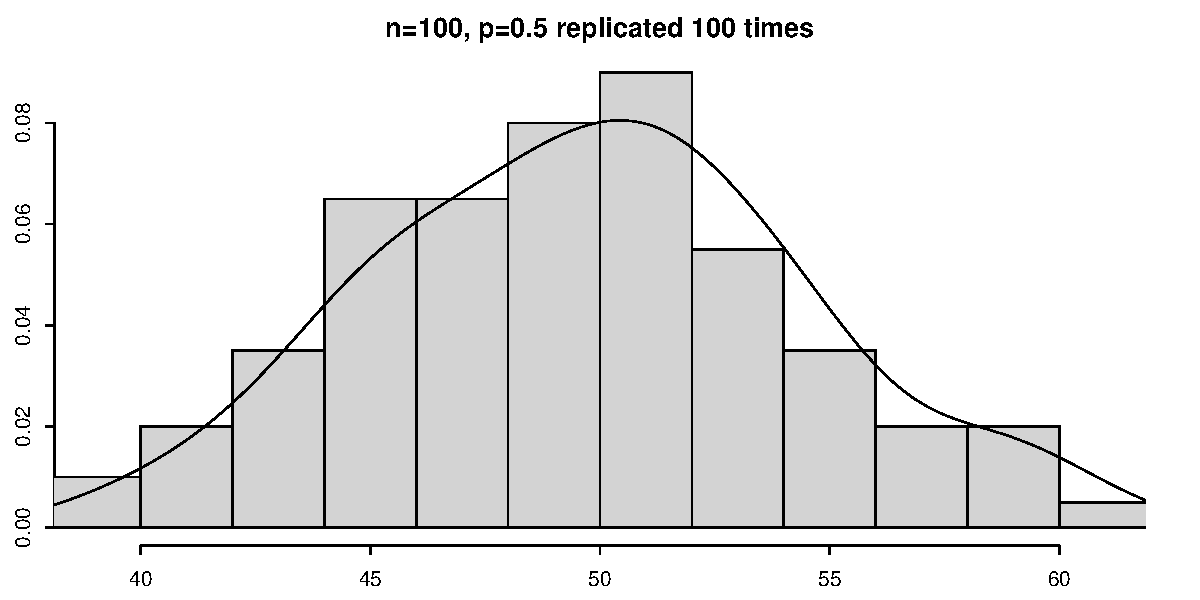
\includegraphics[width=0.89\linewidth]{figure/graphics-unnamed-chunk-5-1} 

}



\end{knitrout}

\end{frame}
%%%%%%%%%%%%%%%%%%%%%%%%%%%%%%%%%%%%%%%%%%%%%%%%%%%%%%%%%%%%

%%%%%%%%%%%%%%%%%%%%%%%%%%%%%%%%%%%%%%%%%%%%%%%%%%%%%%%%%%%%
\begin{frame}[fragile]
%%%%%%%%%%%%%%%%%%%%%%%%%%%%%%%%%%%%%%%%%%%%%%%%%%%%%%%%%%%%

Let us start with a simple example where we repeat the experiment of tossing
$100$ fair coins and recording the number of heads $10000$ times.

\begin{knitrout}\small
\definecolor{shadecolor}{rgb}{1, 1, 1}\color{fgcolor}\begin{kframe}
\begin{alltt}
\hlstd{Y} \hlkwb{<-} \hlkwd{rbinom}\hlstd{(}\hlnum{10000}\hlstd{,} \hlnum{100}\hlstd{,} \hlkwc{p}\hlstd{=}\hlnum{0.5}\hlstd{)}
\hlkwd{summary}\hlstd{(Y)}
\end{alltt}
\begin{verbatim}
   Min. 1st Qu.  Median    Mean 3rd Qu.    Max. 
     32      46      50      50      53      72 
\end{verbatim}
\end{kframe}
\end{knitrout}

\end{frame}
%%%%%%%%%%%%%%%%%%%%%%%%%%%%%%%%%%%%%%%%%%%%%%%%%%%%%%%%%%%%


%%%%%%%%%%%%%%%%%%%%%%%%%%%%%%%%%%%%%%%%%%%%%%%%%%%%%%%%%%%%
\begin{frame}[fragile]
%%%%%%%%%%%%%%%%%%%%%%%%%%%%%%%%%%%%%%%%%%%%%%%%%%%%%%%%%%%%

\begin{knitrout}\small
\definecolor{shadecolor}{rgb}{1, 1, 1}\color{fgcolor}

{\centering 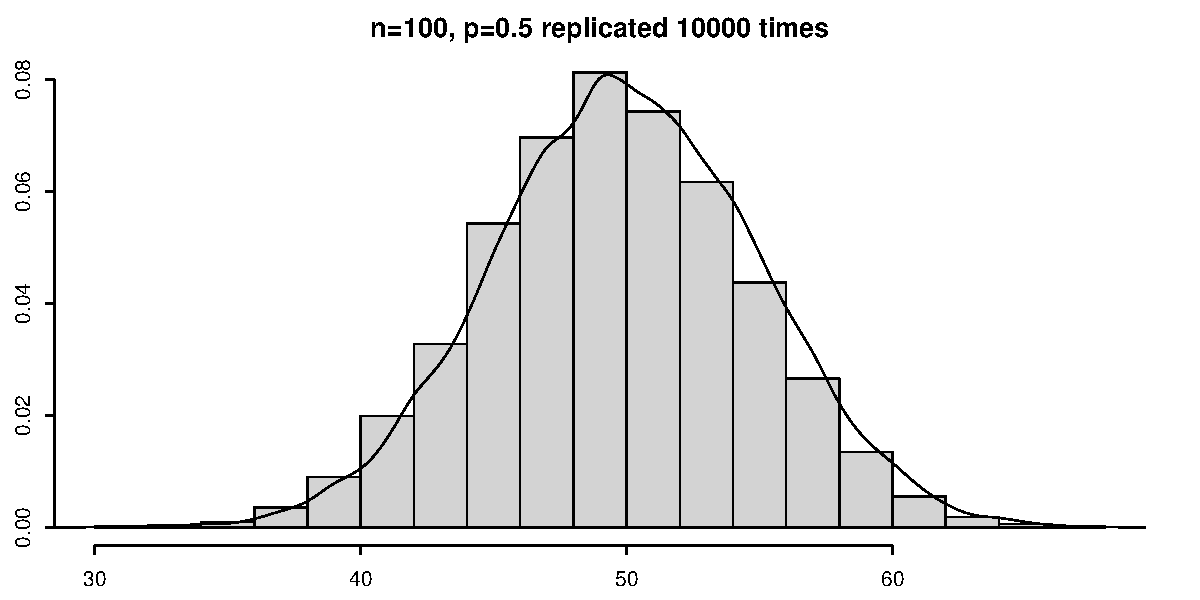
\includegraphics[width=0.89\linewidth]{figure/graphics-unnamed-chunk-7-1} 

}



\end{knitrout}

\end{frame}
%%%%%%%%%%%%%%%%%%%%%%%%%%%%%%%%%%%%%%%%%%%%%%%%%%%%%%%%%%%%

%%%%%%%%%%%%%%%%%%%%%%%%%%%%%%%%%%%%%%%%%%%%%%%%%%%%%%%%%%%%
\begin{frame}[fragile]
%%%%%%%%%%%%%%%%%%%%%%%%%%%%%%%%%%%%%%%%%%%%%%%%%%%%%%%%%%%%

Let us perform the same experiments but instead of observing the number of heads, lets now observe the proportion of heads. First with $10$ repeats

\begin{knitrout}\small
\definecolor{shadecolor}{rgb}{1, 1, 1}\color{fgcolor}\begin{kframe}
\begin{alltt}
\hlstd{Y} \hlkwb{<-} \hlkwd{rbinom}\hlstd{(}\hlnum{10}\hlstd{,} \hlnum{100}\hlstd{,} \hlkwc{p}\hlstd{=}\hlnum{0.5}\hlstd{)}\hlopt{/} \hlnum{100}\hlstd{;}
\hlkwd{summary}\hlstd{(Y)}
\end{alltt}
\begin{verbatim}
   Min. 1st Qu.  Median    Mean 3rd Qu.    Max. 
  0.370   0.435   0.460   0.474   0.515   0.590 
\end{verbatim}
\end{kframe}
\end{knitrout}

\end{frame}
%%%%%%%%%%%%%%%%%%%%%%%%%%%%%%%%%%%%%%%%%%%%%%%%%%%%%%%%%%%%

%%%%%%%%%%%%%%%%%%%%%%%%%%%%%%%%%%%%%%%%%%%%%%%%%%%%%%%%%%%%
\begin{frame}[fragile]
%%%%%%%%%%%%%%%%%%%%%%%%%%%%%%%%%%%%%%%%%%%%%%%%%%%%%%%%%%%%

\begin{knitrout}\small
\definecolor{shadecolor}{rgb}{1, 1, 1}\color{fgcolor}

{\centering 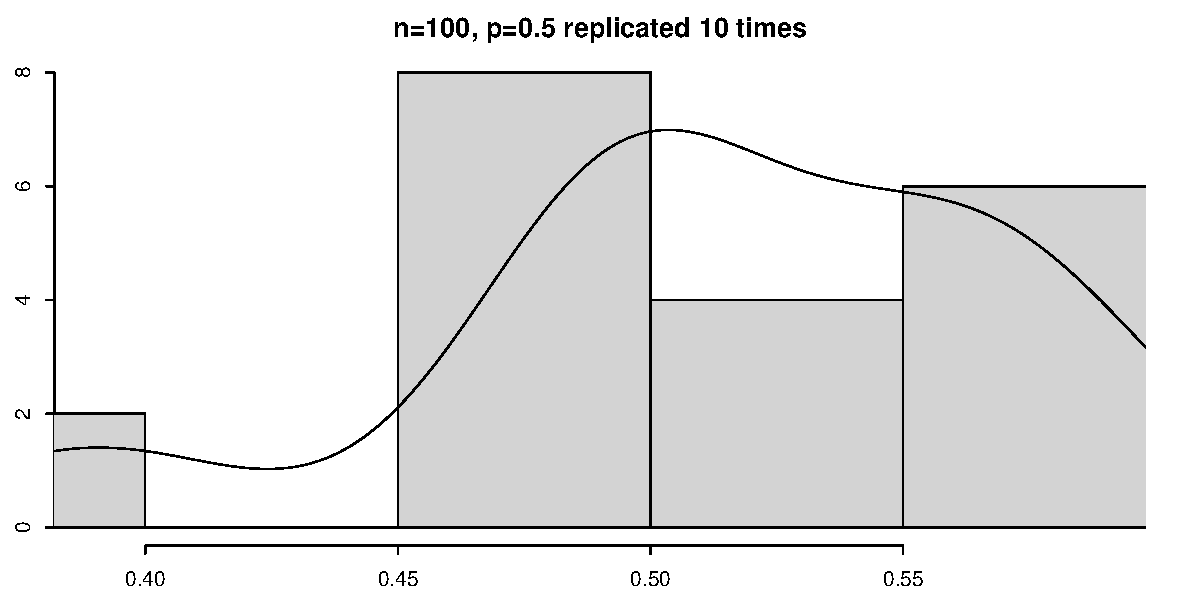
\includegraphics[width=0.89\linewidth]{figure/graphics-unnamed-chunk-9-1} 

}



\end{knitrout}

\end{frame}
%%%%%%%%%%%%%%%%%%%%%%%%%%%%%%%%%%%%%%%%%%%%%%%%%%%%%%%%%%%%


%%%%%%%%%%%%%%%%%%%%%%%%%%%%%%%%%%%%%%%%%%%%%%%%%%%%%%%%%%%%
\begin{frame}[fragile]
%%%%%%%%%%%%%%%%%%%%%%%%%%%%%%%%%%%%%%%%%%%%%%%%%%%%%%%%%%%%

Let us perform the same experiments but instead of observing the number of heads, lets now observe the proportion of heads. First with $100$ repeats

\begin{knitrout}\small
\definecolor{shadecolor}{rgb}{1, 1, 1}\color{fgcolor}\begin{kframe}
\begin{alltt}
\hlstd{Y} \hlkwb{<-} \hlkwd{rbinom}\hlstd{(}\hlnum{100}\hlstd{,} \hlnum{100}\hlstd{,} \hlkwc{p}\hlstd{=}\hlnum{0.5}\hlstd{)}\hlopt{/} \hlnum{100}\hlstd{;}
\hlkwd{summary}\hlstd{(Y)}
\end{alltt}
\begin{verbatim}
   Min. 1st Qu.  Median    Mean 3rd Qu.    Max. 
  0.390   0.460   0.490   0.498   0.530   0.620 
\end{verbatim}
\end{kframe}
\end{knitrout}

\end{frame}
%%%%%%%%%%%%%%%%%%%%%%%%%%%%%%%%%%%%%%%%%%%%%%%%%%%%%%%%%%%%

%%%%%%%%%%%%%%%%%%%%%%%%%%%%%%%%%%%%%%%%%%%%%%%%%%%%%%%%%%%%
\begin{frame}[fragile]
%%%%%%%%%%%%%%%%%%%%%%%%%%%%%%%%%%%%%%%%%%%%%%%%%%%%%%%%%%%%

\begin{knitrout}\small
\definecolor{shadecolor}{rgb}{1, 1, 1}\color{fgcolor}

{\centering 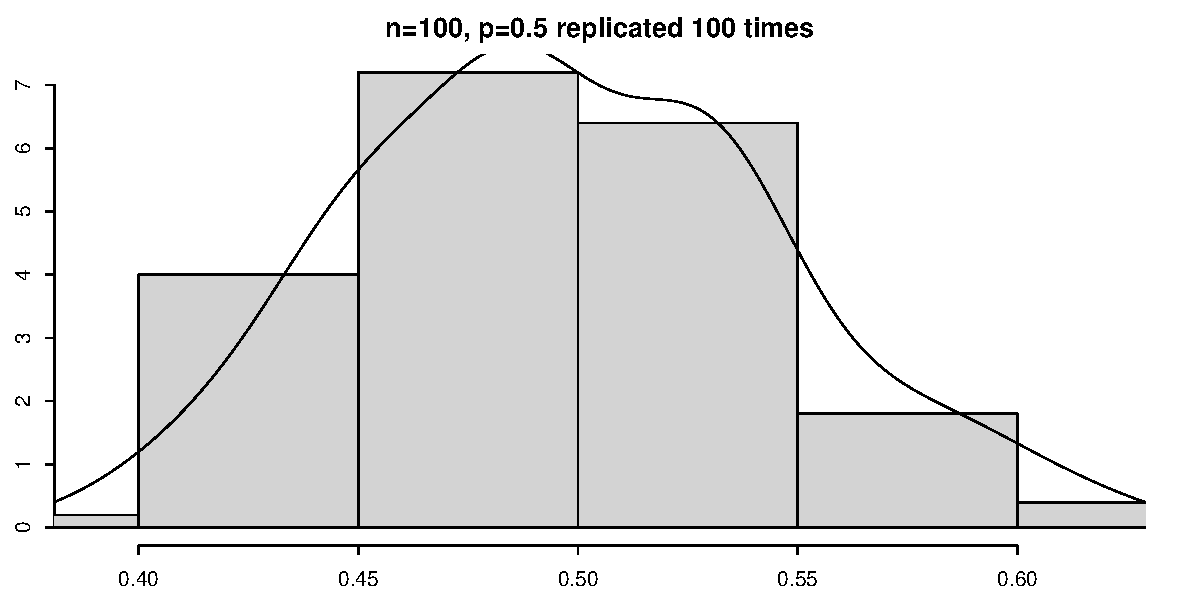
\includegraphics[width=0.89\linewidth]{figure/graphics-unnamed-chunk-11-1} 

}



\end{knitrout}

\end{frame}
%%%%%%%%%%%%%%%%%%%%%%%%%%%%%%%%%%%%%%%%%%%%%%%%%%%%%%%%%%%%


%%%%%%%%%%%%%%%%%%%%%%%%%%%%%%%%%%%%%%%%%%%%%%%%%%%%%%%%%%%%
\begin{frame}[fragile]
%%%%%%%%%%%%%%%%%%%%%%%%%%%%%%%%%%%%%%%%%%%%%%%%%%%%%%%%%%%%

Let us perform the same experiments but instead of observing the number of heads, lets now observe the proportion of heads. First with $10000$ repeats

\begin{knitrout}\small
\definecolor{shadecolor}{rgb}{1, 1, 1}\color{fgcolor}\begin{kframe}
\begin{alltt}
\hlstd{Y} \hlkwb{<-} \hlkwd{rbinom}\hlstd{(}\hlnum{10000}\hlstd{,} \hlnum{100}\hlstd{,} \hlkwc{p}\hlstd{=}\hlnum{0.5}\hlstd{)}\hlopt{/} \hlnum{100}\hlstd{;}
\hlkwd{summary}\hlstd{(Y)}
\end{alltt}
\begin{verbatim}
   Min. 1st Qu.  Median    Mean 3rd Qu.    Max. 
   0.27    0.47    0.50    0.50    0.53    0.70 
\end{verbatim}
\end{kframe}
\end{knitrout}

\end{frame}
%%%%%%%%%%%%%%%%%%%%%%%%%%%%%%%%%%%%%%%%%%%%%%%%%%%%%%%%%%%%

%%%%%%%%%%%%%%%%%%%%%%%%%%%%%%%%%%%%%%%%%%%%%%%%%%%%%%%%%%%%
\begin{frame}[fragile]
%%%%%%%%%%%%%%%%%%%%%%%%%%%%%%%%%%%%%%%%%%%%%%%%%%%%%%%%%%%%

\begin{knitrout}\small
\definecolor{shadecolor}{rgb}{1, 1, 1}\color{fgcolor}

{\centering 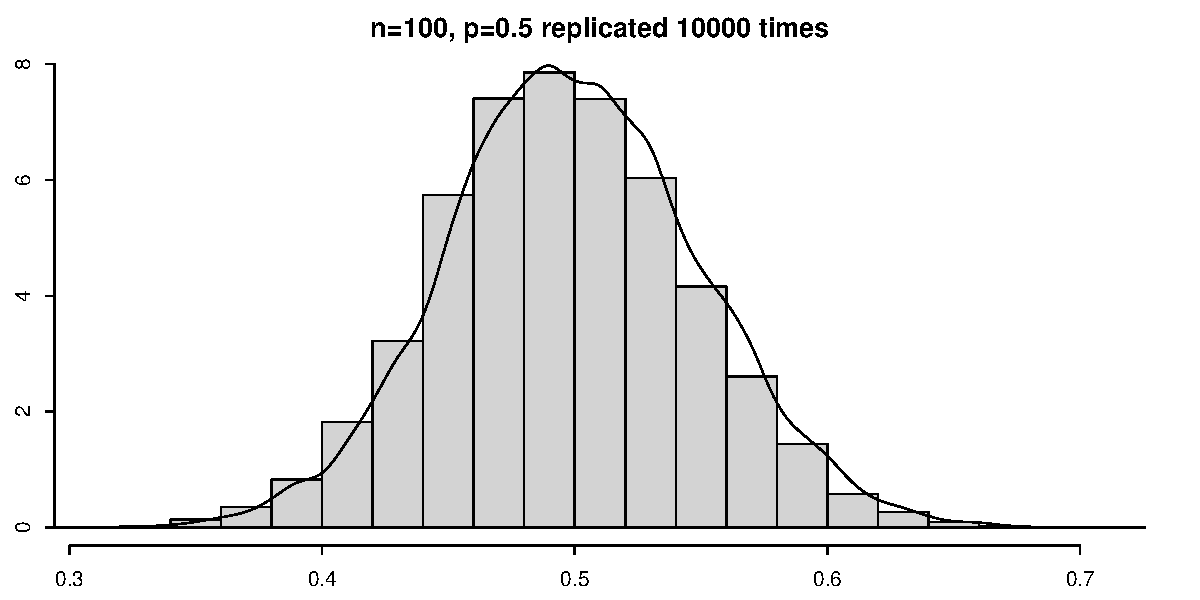
\includegraphics[width=0.89\linewidth]{figure/graphics-unnamed-chunk-13-1} 

}



\end{knitrout}

\end{frame}
%%%%%%%%%%%%%%%%%%%%%%%%%%%%%%%%%%%%%%%%%%%%%%%%%%%%%%%%%%%%

%%%%%%%%%%%%%%%%%%%%%%%%%%%%%%%%%%%%%%%%%%%%%%%%%%%%%%%%%%%%
\begin{frame}[fragile]
%%%%%%%%%%%%%%%%%%%%%%%%%%%%%%%%%%%%%%%%%%%%%%%%%%%%%%%%%%%%

In the previous case, the variables generated were $Bin(100,0.5)$. Now lets look at variables generated at $Bin(20,0.5)$ and repeat the process $10,000$ times.

\begin{knitrout}\small
\definecolor{shadecolor}{rgb}{1, 1, 1}\color{fgcolor}\begin{kframe}
\begin{alltt}
\hlstd{Y1} \hlkwb{<-} \hlkwd{rbinom}\hlstd{(}\hlnum{10000}\hlstd{,} \hlnum{20}\hlstd{,} \hlkwc{p}\hlstd{=}\hlnum{0.5}\hlstd{)}\hlopt{/} \hlnum{20}\hlstd{;}
\hlkwd{summary}\hlstd{(Y1)}
\end{alltt}
\begin{verbatim}
   Min. 1st Qu.  Median    Mean 3rd Qu.    Max. 
   0.10    0.45    0.50    0.50    0.55    0.90 
\end{verbatim}
\end{kframe}
\end{knitrout}

\end{frame}
%%%%%%%%%%%%%%%%%%%%%%%%%%%%%%%%%%%%%%%%%%%%%%%%%%%%%%%%%%%%

%%%%%%%%%%%%%%%%%%%%%%%%%%%%%%%%%%%%%%%%%%%%%%%%%%%%%%%%%%%%
\begin{frame}[fragile]
%%%%%%%%%%%%%%%%%%%%%%%%%%%%%%%%%%%%%%%%%%%%%%%%%%%%%%%%%%%%

\begin{knitrout}\small
\definecolor{shadecolor}{rgb}{1, 1, 1}\color{fgcolor}

{\centering 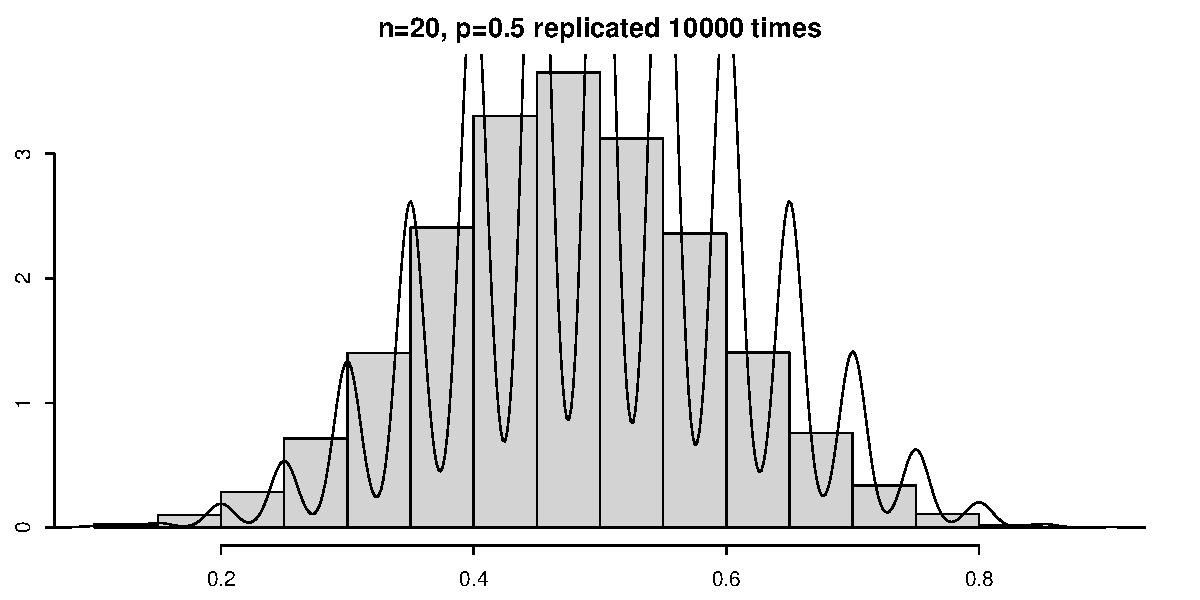
\includegraphics[width=0.89\linewidth]{figure/graphics-unnamed-chunk-15-1} 

}



\end{knitrout}

\end{frame}
%%%%%%%%%%%%%%%%%%%%%%%%%%%%%%%%%%%%%%%%%%%%%%%%%%%%%%%%%%%%

%%%%%%%%%%%%%%%%%%%%%%%%%%%%%%%%%%%%%%%%%%%%%%%%%%%%%%%%%%%%
\begin{frame}[fragile]
%%%%%%%%%%%%%%%%%%%%%%%%%%%%%%%%%%%%%%%%%%%%%%%%%%%%%%%%%%%%

Now lets look at variables generated at $Bin(100,0.5)$ and repeat the process $10,000$ times.

\begin{knitrout}\small
\definecolor{shadecolor}{rgb}{1, 1, 1}\color{fgcolor}\begin{kframe}
\begin{alltt}
\hlstd{Y2} \hlkwb{<-} \hlkwd{rbinom}\hlstd{(}\hlnum{10000}\hlstd{,} \hlnum{100}\hlstd{,} \hlkwc{p}\hlstd{=}\hlnum{0.5}\hlstd{)}\hlopt{/} \hlnum{100}\hlstd{;}
\hlkwd{summary}\hlstd{(Y2)}
\end{alltt}
\begin{verbatim}
   Min. 1st Qu.  Median    Mean 3rd Qu.    Max. 
   0.32    0.47    0.50    0.50    0.53    0.69 
\end{verbatim}
\end{kframe}
\end{knitrout}

\end{frame}
%%%%%%%%%%%%%%%%%%%%%%%%%%%%%%%%%%%%%%%%%%%%%%%%%%%%%%%%%%%%

%%%%%%%%%%%%%%%%%%%%%%%%%%%%%%%%%%%%%%%%%%%%%%%%%%%%%%%%%%%%
\begin{frame}[fragile]
%%%%%%%%%%%%%%%%%%%%%%%%%%%%%%%%%%%%%%%%%%%%%%%%%%%%%%%%%%%%

\begin{knitrout}\small
\definecolor{shadecolor}{rgb}{1, 1, 1}\color{fgcolor}

{\centering 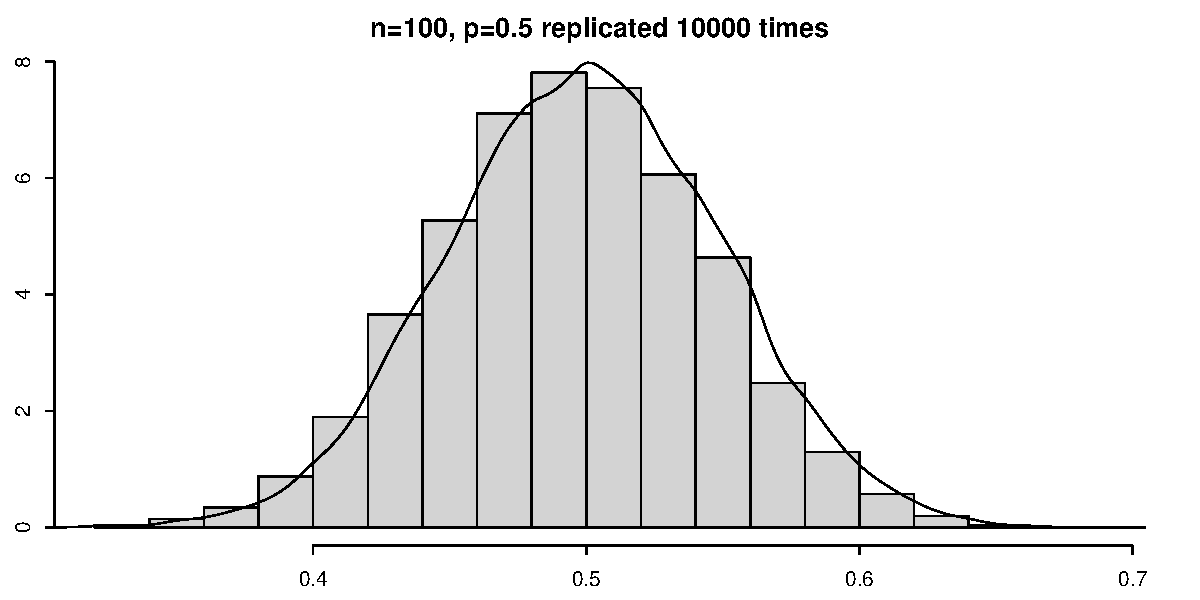
\includegraphics[width=0.89\linewidth]{figure/graphics-unnamed-chunk-17-1} 

}



\end{knitrout}

\end{frame}
%%%%%%%%%%%%%%%%%%%%%%%%%%%%%%%%%%%%%%%%%%%%%%%%%%%%%%%%%%%%

%%%%%%%%%%%%%%%%%%%%%%%%%%%%%%%%%%%%%%%%%%%%%%%%%%%%%%%%%%%%
\begin{frame}[fragile]
%%%%%%%%%%%%%%%%%%%%%%%%%%%%%%%%%%%%%%%%%%%%%%%%%%%%%%%%%%%%

Now lets look at variables generated at $Bin(1000,0.5)$ and repeat the process $10,000$ times.

\begin{knitrout}\small
\definecolor{shadecolor}{rgb}{1, 1, 1}\color{fgcolor}\begin{kframe}
\begin{alltt}
\hlstd{Y3} \hlkwb{<-} \hlkwd{rbinom}\hlstd{(}\hlnum{10000}\hlstd{,} \hlnum{1000}\hlstd{,} \hlkwc{p}\hlstd{=}\hlnum{0.5}\hlstd{)}\hlopt{/} \hlnum{1000}\hlstd{;}
\hlkwd{summary}\hlstd{(Y3)}
\end{alltt}
\begin{verbatim}
   Min. 1st Qu.  Median    Mean 3rd Qu.    Max. 
  0.437   0.489   0.500   0.500   0.511   0.562 
\end{verbatim}
\end{kframe}
\end{knitrout}

\end{frame}
%%%%%%%%%%%%%%%%%%%%%%%%%%%%%%%%%%%%%%%%%%%%%%%%%%%%%%%%%%%%

%%%%%%%%%%%%%%%%%%%%%%%%%%%%%%%%%%%%%%%%%%%%%%%%%%%%%%%%%%%%
\begin{frame}[fragile]
%%%%%%%%%%%%%%%%%%%%%%%%%%%%%%%%%%%%%%%%%%%%%%%%%%%%%%%%%%%%

\begin{knitrout}\small
\definecolor{shadecolor}{rgb}{1, 1, 1}\color{fgcolor}

{\centering 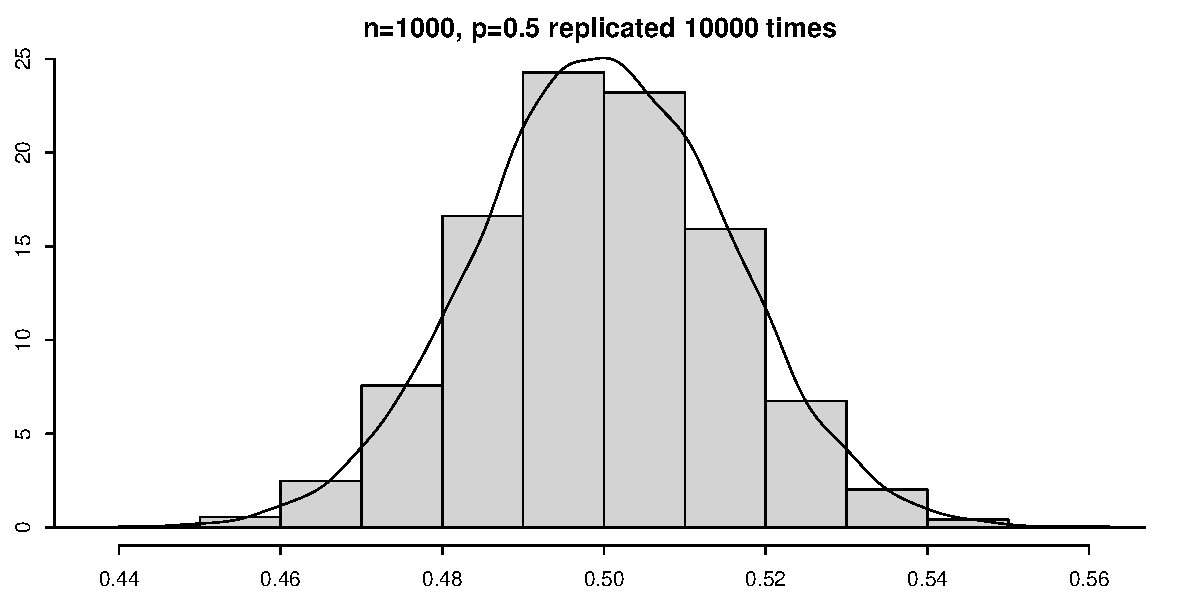
\includegraphics[width=0.89\linewidth]{figure/graphics-unnamed-chunk-19-1} 

}



\end{knitrout}

\end{frame}
%%%%%%%%%%%%%%%%%%%%%%%%%%%%%%%%%%%%%%%%%%%%%%%%%%%%%%%%%%%%


%%%%%%%%%%%%%%%%%%%%%%%%%%%%%%%%%%%%%%%%%%%%%%%%%%%%%%%%%%%%
\begin{frame}[fragile]
%%%%%%%%%%%%%%%%%%%%%%%%%%%%%%%%%%%%%%%%%%%%%%%%%%%%%%%%%%%%

\begin{knitrout}\small
\definecolor{shadecolor}{rgb}{1, 1, 1}\color{fgcolor}

{\centering 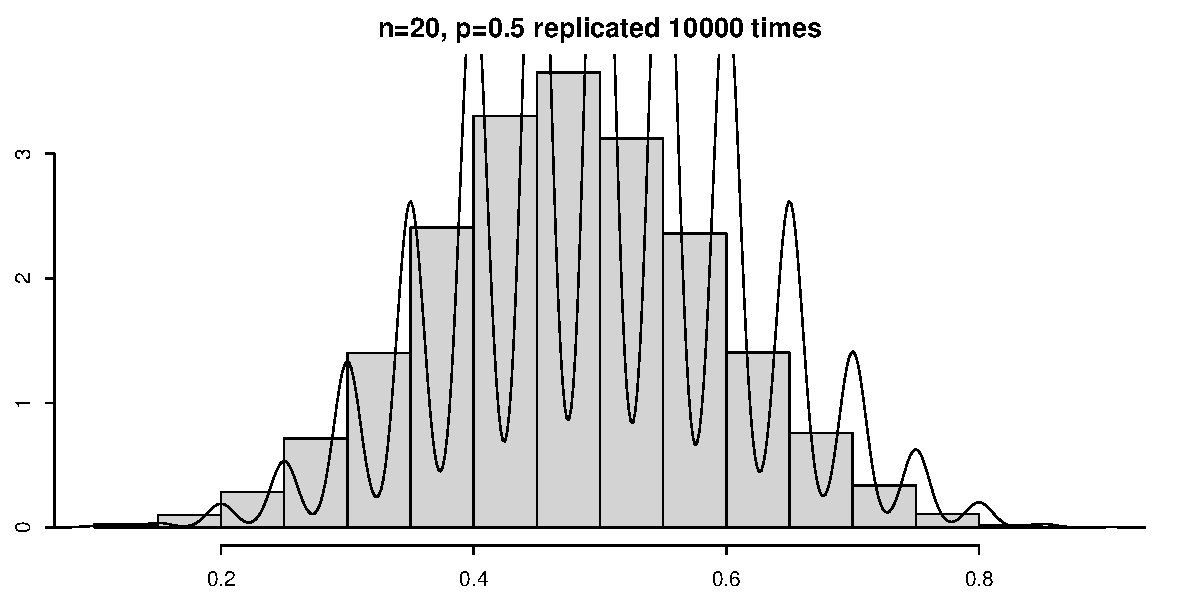
\includegraphics[width=0.89\linewidth]{figure/graphics-unnamed-chunk-20-1} 

}



\end{knitrout}

\end{frame}
%%%%%%%%%%%%%%%%%%%%%%%%%%%%%%%%%%%%%%%%%%%%%%%%%%%%%%%%%%%%

%%%%%%%%%%%%%%%%%%%%%%%%%%%%%%%%%%%%%%%%%%%%%%%%%%%%%%%%%%%%
\begin{frame}[fragile]
%%%%%%%%%%%%%%%%%%%%%%%%%%%%%%%%%%%%%%%%%%%%%%%%%%%%%%%%%%%%

\begin{knitrout}\small
\definecolor{shadecolor}{rgb}{1, 1, 1}\color{fgcolor}

{\centering 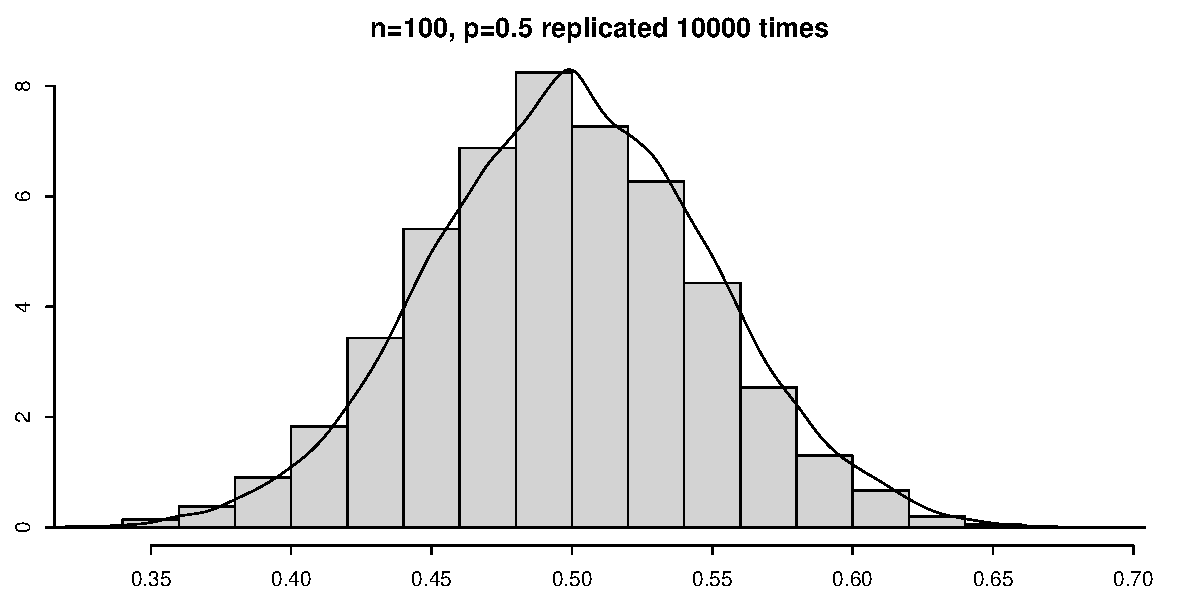
\includegraphics[width=0.89\linewidth]{figure/graphics-unnamed-chunk-21-1} 

}



\end{knitrout}

\end{frame}
%%%%%%%%%%%%%%%%%%%%%%%%%%%%%%%%%%%%%%%%%%%%%%%%%%%%%%%%%%%%

%%%%%%%%%%%%%%%%%%%%%%%%%%%%%%%%%%%%%%%%%%%%%%%%%%%%%%%%%%%%
\begin{frame}[fragile]
%%%%%%%%%%%%%%%%%%%%%%%%%%%%%%%%%%%%%%%%%%%%%%%%%%%%%%%%%%%%

\begin{knitrout}\small
\definecolor{shadecolor}{rgb}{1, 1, 1}\color{fgcolor}

{\centering 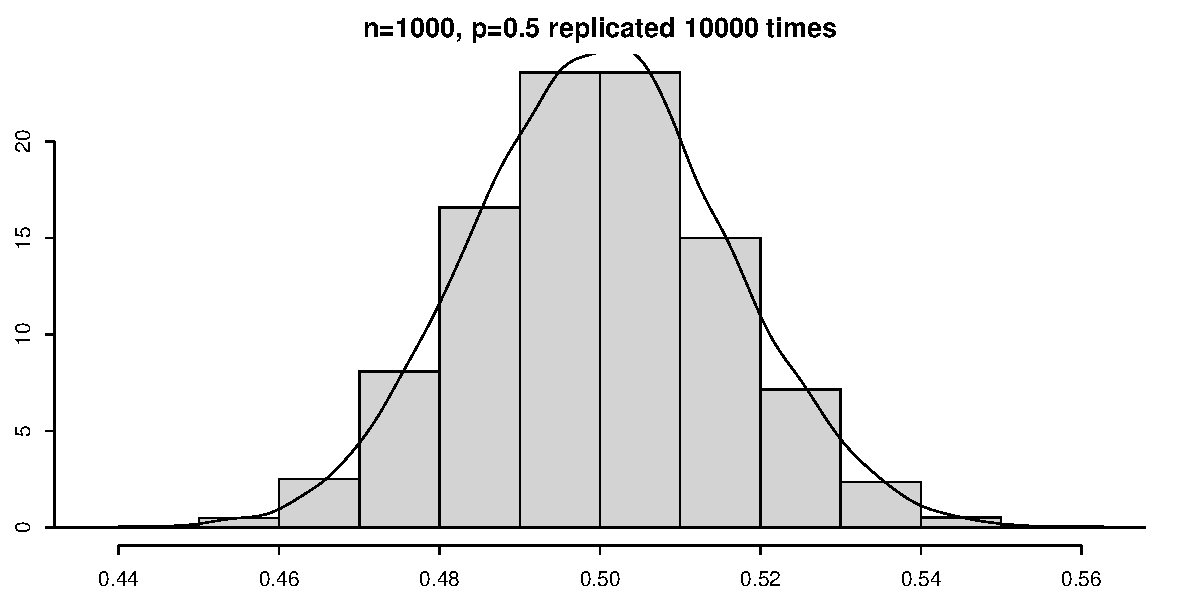
\includegraphics[width=0.89\linewidth]{figure/graphics-unnamed-chunk-22-1} 

}



\end{knitrout}

\end{frame}
%%%%%%%%%%%%%%%%%%%%%%%%%%%%%%%%%%%%%%%%%%%%%%%%%%%%%%%%%%%%

%%%%%%%%%%%%%%%%%%%%%%%%%%%%%%%%%%%%%%%%%%%%%%%%%%%%%%%%%%%%
\begin{frame}[fragile]
%%%%%%%%%%%%%%%%%%%%%%%%%%%%%%%%%%%%%%%%%%%%%%%%%%%%%%%%%%%%
\frametitle{Take home message}

The distribution of $\bar{X}$ seems to be more concentrated as we increase the number of tosses per experiment from $n=20$ to $n=100$ to $n=1000$. This is because 

$$ var(\bar{X}_{n}) = \frac{p(1-p)}{n} = \frac{0.5 \times 0.5}{n} = \frac{0.25}{n} $$

So as $n$ increases, variance decreases. Also note $\bar{X}$ being unbiased for any $n$ for the probability of success $p=0.5$. 

$$ E(\bar{X}_{n}) = 0.5 $$

As a result, all the histograms are centered around $0.5$.

\end{frame}
%%%%%%%%%%%%%%%%%%%%%%%%%%%%%%%%%%%%%%%%%%%%%%%%%%%%%%%%%%%%

%%%%%%%%%%%%%%%%%%%%%%%%%%%%%%%%%%%%%%%%%%%%%%%%%%%%%%%%%%%%
\begin{frame}[fragile]
%%%%%%%%%%%%%%%%%%%%%%%%%%%%%%%%%%%%%%%%%%%%%%%%%%%%%%%%%%%%
\frametitle{Take home message}

If we repeat the experiment a large number of times, the distribution seems to behave like a Normal distribution for both the proportion of successes $\bar{X}$ and $\sum_{i=1}^{n} X_i$. \pause \newline

The distribution is centered at mean $0.5$ for $\bar{X}$ with spread $\frac{0.25}{n}$ and at $n \times 0.5$ for $\sum_{i=1}^{n} X_i$ with variance $n \times 0.25$. \pause \newline

This phenomenon is called Central Limit Theorem (CLT). 

\end{frame}
%%%%%%%%%%%%%%%%%%%%%%%%%%%%%%%%%%%%%%%%%%%%%%%%%%%%%%%%%%%%

%%%%%%%%%%%%%%%%%%%%%%%%%%%%%%%%%%%%%%%%%%%%%%%%%%%%%%%%%%%%
\begin{frame}[fragile]
%%%%%%%%%%%%%%%%%%%%%%%%%%%%%%%%%%%%%%%%%%%%%%%%%%%%%%%%%%%%
\frametitle{Central Limit Theorem}

More generally if $X_1, X_2, \cdots, X_n$ be independent identically distributed (iid) random variables coming from an experiment with mean $\mu$ and variance $\sigma^2$, 

$$ E(X_i) = \mu \hspace{0.5 cm} var(X_i) = \sigma^2 $$

then 

$$ \sum_{i=1}^{n} X_{i} \approx N \left (n \mu, n \sigma^2 \right )  $$

and 

$$ \frac{1}{n}\sum_{i=1}^{n} X_{i} \approx N \left (\mu, \frac{\sigma^2}{n} \right ) $$

As a result if you repeat the experiment many many times and plot the histogram, the hitogram can be approximated by a normal distribution with these means and variance structure.

\end{frame}
%%%%%%%%%%%%%%%%%%%%%%%%%%%%%%%%%%%%%%%%%%%%%%%%%%%%%%%%%%%%

%%%%%%%%%%%%%%%%%%%%%%%%%%%%%%%%%%%%%%%%%%%%%%%%%%%%%%%%%%%%
\begin{frame}[fragile]
%%%%%%%%%%%%%%%%%%%%%%%%%%%%%%%%%%%%%%%%%%%%%%%%%%%%%%%%%%%%
\frametitle{Central Limit Theorem for Bernoulli}

More generally if $X_1, X_2, \cdots, X_n$ be independent identically distributed (iid) $Ber(p)$ random variables coming from an experiment with parameter $p$, meaning mean $p$ and variance $p(1-p)$, 

$$ E(X_i) = p \hspace{0.5 cm} var(X_i) = p(1-p) $$

then 

$$ \sum_{i=1}^{n} X_{i} \approx N \left (np, np(1-p) \right ) \hspace{0.5 cm} n \;\; large $$

and 

$$ \frac{1}{n}\sum_{i=1}^{n} X_{i} \approx N \left (p, \frac{p(1-p)}{n} \right )  \hspace{0.5 cm} n \;\; large $$

As a result if you repeat the experiment many many times and plot the histogram, the hitogram can be approximated by a normal distribution with these means and variance structure.

\end{frame}
%%%%%%%%%%%%%%%%%%%%%%%%%%%%%%%%%%%%%%%%%%%%%%%%%%%%%%%%%%%%

%%%%%%%%%%%%%%%%%%%%%%%%%%%%%%%%%%%%%%%%%%%%%%%%%%%%%%%%%%%%
\begin{frame}[fragile]
%%%%%%%%%%%%%%%%%%%%%%%%%%%%%%%%%%%%%%%%%%%%%%%%%%%%%%%%%%%%
\frametitle{Binomial approximated by Normal}

$$ \sum_{i=1}^{n} X_{i} \approx N \left (np, np(1-p) \right ) \hspace{0.5 cm} n \;\; large $$

But we know that for any $n$, 

$$\sum_{i=1}^{n} X_i \sim  Bin(n,p)$$ \pause \newline

So this is a normal approximation to Binomial distribution. \pause \newline

Wait!! \pause \newline

A continuous distribution approximating a Discrete distribution??  

How to map discrete probabilities to continuous densities?

\end{frame}
%%%%%%%%%%%%%%%%%%%%%%%%%%%%%%%%%%%%%%%%%%%%%%%%%%%%%%%%%%%%

%%%%%%%%%%%%%%%%%%%%%%%%%%%%%%%%%%%%%%%%%%%%%%%%%%%%%%%%%%%%
\begin{frame}[fragile]
%%%%%%%%%%%%%%%%%%%%%%%%%%%%%%%%%%%%%%%%%%%%%%%%%%%%%%%%%%%%
\frametitle{Continuity Correction}

\begin{tabular}{|c|c|}
\hline
Discrete & Continuous \\ \hline
$X=3$ & $2.5 < X < 3.5$ \\ \hline
$X > 3$ & $X > 3.5$ \\ \hline
$X \geq 3$ & $ X > 2.5 $ \\ \hline
$X < 3$ & $X < 2.5$ \\ \hline
$X \leq 3$ & $X < 3.5$ \\ \hline
\end{tabular}

\end{frame}
%%%%%%%%%%%%%%%%%%%%%%%%%%%%%%%%%%%%%%%%%%%%%%%%%%%%%%%%%%%%

\end{document}



